% Chapter 3

\chapter{Mirativity and obviousness as intonational meanings} % 
%Chapter title
\label{ch:3} % For referencing the chapter elsewhere, use \chapref{ch:mathtest}



To solve some of the inconsistencies we encountered in our review of the literature on Spanish intonation in Chapters~\ref{ch:1} and~\ref{ch:2}, we need to take a step back and reflect on intonational meaning more generally. That is what we will do in this chapter, before returning to the investigation of Spanish intonation from \chapref{ch:4} onward.

What does it mean when we link intonation to notions such as declarative, interrogative, imperative, and vocative? First and foremost, it means that we link it to speech acts \citep{Austin.1962,Searle.1969}. Speech acts can be seen as moves in a \textit{Sprachspiel} `language game' \citep{Wittgenstein.2009}. These moves take propositions, expressed by sentence radicals, and use them to change the state of the game \citep[62--66]{Krifka.2014}. Yet apart from speech acts, there are distinctions in \autoref{tab:intonationalcategoriesPRIETO} that 
do not fall squarely within such a view. \textit{Obviousness}, 
(\textit{counter})\textit{expectation}, \textit{uncertainty}, 
\textit{insistence}, and \textit{echo} are notions that seem to have an impact on intonation, yet they are not easily captured in terms of speech acts. 

One solution to this problem is to simply exclude them from our analysis 
by interpreting them as emotive flavors added to the grammatically 
relevant distinctions. Instead of representing systematic linguistic 
choices, they would express the state of arousal or degree of emphasis of a speaker in an extralinguistic way. An alternative approach is to 
model the meanings behind these labels based on the observation of phenomena that lend themselves for comparison (such as particles and syntactic structures). This allows us to predict possible combinations and mutually exclusive meanings. Such models can then guide empirical research that discerns whether the individual meanings are encoded by prosody, or by other grammatical means, or are not reliably encoded at all in a specific language or variety.

Let's recapitulate \autoref{tab:intonationalcategoriesPRIETOsmall}. The first two categories, neutral broad focus 
statements and contrastive focus statements, mirror the extensive literature on the relation between focus and prosody. Even though there is 
disagreement between Tables~\ref{tab:intonationalcategoriesPRIETOsmall} and 
\ref{tab:intonationalcategoriesGABRIEL} about the tonal association of 
the H target in contrastive focus conditions (L* HL\% vs. LH* L\%), both 
analyses agree in that contrastive focus is a relevant category for the 
intonational phonology of Spanish. Exclamative statements, obviousness 
statements, and insistent explanations, on the other hand, present us with 
a series of meanings that have only recently been added to the discussion on \ac{IS} in Spanish and are therefore not represented in \autoref{tab:intonationalcategoriesGABRIEL}. By putting them at the center 
of our discussion, I attempt a decompositional approach to intonational meaning in Spanish. 

Throughout this chapter and the following investigation, I ask the same 
questions for each sentence type: Is it possible to decompose the meanings that give 
rise to its interpretation? And if so, is there a way to express some of 
these individual meanings with intonation only? Based on work by \citet{Kratzer.1991,Kratzer.2012}, \citet{ZanuttiniPortner2003}, \citet{Potts.2007expressivedimension}, \citet{FarkasBruce.2010}, \citet{BianchiBocciCruschina.2016}, \citet{Roberts.2017}, \citet{Reich.2018}, and \citet{Rett.2021emotivemarkers}, the main argument is that there are several layers of meaning at play in the determination of the prosodic form of a turn. Apart from the basic distinction between assertion and interrogation, these are focus-background structure, interactive stances of (dis)agreement, and evaluative modal meaning. %These meanings are separate from , and should also be separated from the scalar implicatures often associated with exclamatives.%\footnote{Non-at-issue meaning (also called projective meaning, \cite{BeaverRobertsSimonsTonhauser.2017}) includes conventional implicatures and presuppositions. Conventional implicatures ``quietly \textit{impose} their content on the Common Ground'' (\cite[32]{Potts.2015}), whereas presuppositions require that $p$ be in the Common Ground to be felicitous. They are \textit{non-at-issue} in the sense that they cannot be challenged directly with `\textit{No! I don't agree with \ldots!}' but only with moves like `\textit{Oh, so \ldots?}' or `\textit{Wait a minute, is it the case that \ldots?}' which do not target the current \ac{QUD} (\cite{Taniguchi.2017}, \cite[259]{Westera.2017}; pace \cite[414]{Rett.2011}). 
	
%Intonational meaning is difficult to be made at-issue (\ref{ex:atisssueintonation}) and needs to be challenged even more explicitly (\ref{ex:challangeintonation}) than lexical presuppositions (\ref{ex:challangepresupposition}). 
	
%\begin{exe}
%		\ex \label{ex:atisssueintonation} 
%		A: Did you expect climate change to affect you?\\
%		B: *Climate change is affecting me! $\downarrow$ (reading: No, I didn't expect it.)\\
%		B: Climate change is affecting me!? $\uparrow$ (reading: It doesn't affect me.)	
%\end{exe}
	
%\begin{exe}
%		\ex \label{ex:challangepresupposition} 
%		A: He didn't finish the marathon. \\
%		B: No, he didn't even start.
%\end{exe}
	
%\begin{exe}
%		\ex \label{ex:challangeintonation} 
%		A: He finished the marathon! $\downarrow$ (reading: I didn't expect it.)\\
%		B: *No, that was expectable. He's a prodigy. \\
%		B: Wait a minute\ldots You didn't expect that? He's a prodigy.	
%\end{exe}
%} 

\section{Decomposing exclamatives}
\label{ch:3.1}

\subsection{Exclamatives in perspective}
\label{ch:3.1.1}

The basic assumption underlying most of the literature on exclamatives in 
Spanish and many other languages is that \textit{wh}-exclamatives are a kind of 
exclamative prototype. In English, \textit{wh}-exclamatives 
(\ref{ex:exclamativaWH}a) can be distinguished from \textit{wh}-questions (\ref{ex:exclamativaWH}b) because they lack an auxi\-liary and therefore have no sub\-ject-auxi\-liary inversion. Yet in Spanish and other Romance languages 
(see \cite{KellertETAL.2018} for Cosenza Italian), only prosody 
distinguishes between the two in the absence of disambiguating lexical 
material (\ref{ex:exclamativaWH}c,d).\footnote{Note that adverbs of 
quantity such as \textit{tan} `so' as well as 
definite countable nouns with the \textit{wh}-pronoun in specifier position are 
ungrammatical in questions, whereas do-support is ungrammatical in \textit{wh}-exclamatives.}

\begin{exe} 
\ex \label{ex:exclamativaWH}
\begin{xlist}
	
	\ex What spicy food she eats!
	\ex What spicy food does she eat?
	\ex ¡Qué comida picante come!
		\glt `What spicy food (s)he eats!'
	\ex ¿Qué comida picante come?
		\glt `What spicy food does (s)he eat?'
\end{xlist}
\end{exe}

Yet \textit{wh}-exclamatives are far from being the only candidates for 
exclamative intonation. Interjective syntactic groups 
(\ref{ex:exclamacionexclamativa}a), exclamative groups 
(\ref{ex:exclamacionexclamativa}b), quantificational expressions 
(\ref{ex:exclamacionexclamativa}c), particle-infinitive 
constructions with \textit{mira} `look' 
(\ref{ex:exclamacionexclamativa}d), and so-called ``hidden 
exclamatives'' (\ref{ex:exclamacionexclamativa}e) also deserve to be 
mentioned \parencites[5]{Bosque.2017}[811]{RealAcademiaEspanola.2010}[144]{Villalba.2017}.

\begin{exe} 
\ex \label{ex:exclamacionexclamativa}
\begin{xlist}
	\ex ¡Caramba con el muchachito! 
	\glt `Damn, what a guy!'
	
	\ex ¡Menuda suerte!
	\glt `What luck!' 
	
	\ex ¡Vaya si me gusta!
	\glt `Boy do I like it!'
	
	\ex ¡Mira que haber dejado tu empleo! 
	\glt `I can't believe you left your job!'
	
	\ex ¡El chico es de travieso! 
	\glt `They boy is so naughty!' 
\end{xlist}
\end{exe}

What all these written examples have in common is the fact that they make use of the graphemes 〈¡〉 and 〈!〉, the Spanish exclamation marks. They are 
counted as cases of primary exclamatives, as opposed to ``intonation only'' 
cases with declarative syntax (\ref{ex:exclamacionDECLARATIVA}a), which 
are either labeled as ``secondary'' \citep[7]{Bosque.2017} or as 
grammatically irrelevant \citep{Olbertz.2012} since they are syntactically 
and lexically identical with declarative sentences 
(\ref{ex:exclamacionDECLARATIVA}b).

\begin{exe} 
	\ex \label{ex:exclamacionDECLARATIVA}
	\begin{xlist}
	\ex ¡Come comida picante!
	\glt `(S)he eats spicy food!'
	
	\ex Come comida picante.
	\glt `(S)he eats spicy food.'
	\end{xlist}
\end{exe}

The main argument of this section is that dismissing ``intonation only'' 
cases from our analysis is damaging to our understanding of both intonation 
in general and the sentence types commonly discussed as syntactically 
encoded ``primary'' exclamatives. Only by comparing the prosodic 
variability of both \textit{wh}-exclamatives and ``intonation only'' exclamatives is it possible to determine the role of intonation in both of them.

The nuclear contour of \textit{wh}-exclamatives such as 
(\ref{ex:exclamativaWH}c) is described as L$+$¡H* L\%, that is, an 
upstepped early rising pitch 
accent followed by a low \ac{IP} boundary (see \autoref{tab:intonationalcategoriesPRIETOsmall}). This nuclear intonation is 
also found in echo yes-no questions, but it is different from an L$+$H* 
L!H\% in statements of the obvious. 

Semantically, two types of exclamatives have received an in-depth, decompositional analysis: degree exclamatives and polar exclamatives. While most of the literature on the syntax and semantics of exclamatives has dealt with degree exclamatives such as (\ref{ex:whexclamativeINTRO}), \citet{Grosz.2012} can be credited with having shifted the focus towards polar exclamatives such as (\ref{ex:dassexclamativeINTRO}). Yet in both strands in the literature, prosody has been largely neglected as a factor. In the following, I shall compare the influential approach by \citet{ZanuttiniPortner2003} with the unified treatment of polar exclamatives and optatives in \citet{Grosz.2012}. En route, we will learn about the potential of semantic decomposition of exclamatives, while also appreciating the limiting effect of neglecting prosody on the understanding of exclamatives.

\begin{exe}
	\ex German\label{ex:dassexclamativeINTRO}\\ Mensch, dass Sie hier sind!
	\glt `Man, that you are here!'
	
	\ex \label{ex:whexclamativeINTRO} Wie schön er ist!
	\glt `How beautiful he is!' 
\end{exe}


According to \citet[26]{Grosz.2012} ``degree exclamatives express amazement at the degree to which something holds; they typically involve some gradable property, and often take the shape of wh-clauses''. \citet[15,16]{ZanuttiniPortner2003} analyze \textit{wh}-exclamative clauses as 
denoting two abstract features: \textit{widening} of a scalarly ordered 
domain (\ref{ex:ZanuttiniPortnerWIDENING}) 
and presupposed \textit{factivity} of the proposition denoted by the root 
sentence (\ref{ex:ZanuttiniPortnerFACTIVITY}). The definition of 
\textit{widening} is to be read as adding to an ascendingly 
ordered ($\prec$) domain of reference an object 
(\ref{ex:ZanuttiniPortnerWIDENING}a) which supersedes 
the rank of any object of the domain (\ref{ex:ZanuttiniPortnerWIDENING}b).\footnote{Note that \citet{ZanuttiniPortner2003} use * for ungrammaticality instead of \#, which I use here and in all following examples for turns deemed unacceptable either by me or other researchers. This is meant both as a precaution against taking individual acceptability judgments as universal (in the absence of controlled perceptual tests) and to avoid confusion with \ac{ToBI} pitch accent notation.} In natural language, (\ref{ex:exclamativaWH}a,c) would read `(s)he eats food that is more spicy than what would fall under grades of spiciness'.
The test applied by \citet{ZanuttiniPortner2003} for this relation is the impossibility of embedding an 
exclamative sentence under certain negated verbs of wonder or amazement 
(\ref{ex:ZanuttiniPortnerNOTAMAZING}). This is explained by an 
incompatibility between a scalar implicature of the exclamative and the 
denying of the predicate \textit{amazing}, which according to them denotes the 
same \textit{widening} relation \citep[21]{ZanuttiniPortner2003}. 
Crucially, though, this effect does not hold if it is possible to separate 
the speaker's domain of expected scalar values from the expectations of 
the subject of the matrix sentence (\ref{ex:ZanuttiniPortnerNOTAMAZED}). This is explained by the fact that 
(\ref{ex:ZanuttiniPortnerNOTAMAZING}) denies the existence of (or 
difference between) two ordered domains, whereas 
(\ref{ex:ZanuttiniPortnerNOTAMAZED}) only denies such a domain difference 
for the subject of the sentence.

\begin{exe}
	\judgewidth{\#}
	\ex \label{ex:ZanuttiniPortnerWIDENING}Widening:\\
	For any clause S marked by $R_{\textit{widening}}$, widen the 
	initial domain, D1, to a new domain, D2, such that
	\begin{xlist}
		\ex $ \llbracket S \rrbracket_{D2,\prec} - \llbracket S 
		\rrbracket_{D1,\prec} \neq \varnothing $ and 
		\ex $\forall x \forall y [(x\in $ D1 \& y $\in ($D2$-$D1$)) 
		\rightarrow x \prec y] $.
	\end{xlist}
	\ex[\#]{\label{ex:ZanuttiniPortnerNOTAMAZING}It's not amazing how 
	(very) tall he is.}

	\ex[]{\label{ex:ZanuttiniPortnerNOTAMAZED}She is not amazed at how 
	(very) tall he is.}
\end{exe}

The property of \textit{factivity}, on the other hand, can be seen in that it is 
impossible to deny knowledge about the content of an exclamative 
(\ref{ex:ZanuttiniPortnerDONTKNOW}). Moreover, it is impossible to answer 
a question with an exclamative (\ref{ex:ZanuttiniPortnerANSWER}), a fact 
that is expected under the presuppositional analysis given that answers 
may never presuppose the information that the question asked about (\ref{ex:ZanuttiniPortnerANSWER2}). The definition of \textit{factivity} 
(\ref{ex:ZanuttiniPortnerFACTIVITY}) is to be 
read as requiring a presupposition of truth for every proposition that is 
an element of the difference in sentence denotation $\llbracket S 
\rrbracket$ between a widened and an unwidened domain.

\begin{exe} 
	\ex \label{ex:ZanuttiniPortnerFACTIVITY} Factivity: \\
	For any clause S marked by $R_{\textit{factivity}}$, every $p \in 
	\llbracket S \rrbracket_{D2,\prec} - \llbracket $S$ 
	\rrbracket_{D1,\prec}$ is presupposed to be true.

	\ex[\#]{\label{ex:ZanuttiniPortnerDONTKNOW}I don't know how very 
	tall he is.}

	\ex \label{ex:ZanuttiniPortnerANSWER} 
		\begin{xlist}[A:]
			\exi{A:}[]{Is he tall?}
			\exi{B:}[\#]{How tall he is.}
		\end{xlist}

	\ex \label{ex:ZanuttiniPortnerANSWER2} 
		\begin{xlist}[A:]
			\exi{A:}[]{Did Bill leave?}
			\exi{B:}[\#]{It's odd that he did.}
		\end{xlist}
\end{exe}

At first glance, the arguments for presupposed factivity hold equally well 
for Spanish. Neither is it possible to embed exclamatives under negated 
verbs of knowing (\ref{ex:ZPspanishDONTKNOW}), nor can they be used as 
answers (\ref{ex:ZPspanishANSWER}). 

\begin{exe} 
	\ex[\#]{\label{ex:ZPspanishDONTKNOW}No sé ¡qué (tan) alto es!
	\glt `I don't know how (very) tall (s)he is!'}
	\ex \label{ex:ZPspanishANSWER} 
	\begin{xlist}
		\exi{A:}[]{¿Es alta? \glt `Is she tall?'}
		\exi{B:}[\#]{¡Qué (tan) alta es! \glt `How (very) tall she is!'}
	\end{xlist}
\end{exe}

Yet Spanish orthography hints at a 
problem less easily visible in English: exclamatives, if marked by 
exclamation marks, cannot be embedded at all 
(\ref{ex:ZPspanishEMBED}).\footnote{See \citet[244]{FarkasRoelofsen.2017} for a similar argument for English rising declaratives.} We cannot apply the 
intonational marking for exclamation to the embedded sentence only. Either the entire complex sentence is marked with exclamation marks (\ref{ex:ZPspanishEMBED2}), which seems like a dubious case to me, or with a full stop (\ref{ex:ZPspanishEMBED3}). Instead, a different construction (lo + \ac{AP} + que + VP) has to be used 
(\ref{ex:ZPspanishEMBED4}) (see \cite[229]{GarciaGarcia.2018} 
for examples of such adjective phrase exclamatives).

\begin{exe}
	\judgewidth{?\#}
	\ex[\#]{\label{ex:ZPspanishEMBED}Ya sé ¡qué (tan) alto es!
			\glt `I know already how (very) tall (s)he is!'}
	\ex[?\#]{\label{ex:ZPspanishEMBED2}¡Ya sé qué alto es!
			\glt`I know already how (very) tall (s)he is!'}
	\ex[]{\label{ex:ZPspanishEMBED3}Ya sé qué alto es.
			\glt `I know already how (very) tall (s)he is.'}
	\ex[]{\label{ex:ZPspanishEMBED4} Ya sé lo alto que es.
			\glt `I know already how (very) tall (s)he is.'}
\end{exe}

Given the reduced amount of prosodic scope information encoded by 
exclamation marks in English, which simply do not indicate the beginning 
of a prosodic domain, written examples such as 
(\ref{ex:ZanuttiniPortnerNOTAMAZED}) give the illusion of a stable 
illocutionary meaning in both embedded and unembedded exclamatives. The lack 
of interest in prosodic features has led to the assumption that the features of syntax (or their meanings) impede the embedding of exclamatives. Yet I take this effect to be caused by an additional level of meaning, which is encoded by intonation. To understand exclamatives, or any other sentence type \citep{Reich.2008}, it is necessary to disentangle the contribution of intonation from that of syntax and other markers.

Turning to polar exclamatives, Grosz states that they ``are utterances that express surprise, shock or amazement at a fact (not at the degree to which something holds) without a lexical item that means surprise, shock or amazement'' \citep[25]{Grosz.2012}. In that respect, they could be called mirative insubordinates.\footnote{Miratives denote a ``semantic category of new or unassimilated information'' \citep[533]{DeLancey.2012} and have been found to be a grammatical category in a variety of languages \citep{HengeveldOlbertz.2012}. Further examples are provided in \sectref{ch:3.3.3}.} They have been described for German and other Germanic languages such as Swedish as exclamatives introduced by a complementizer corresponding to \textit{that}, yet without a subordinating effect (\ref{ex:dassexclamative}). They differ from degree exclamatives (\ref{ex:whexclamativeungradable}) in allowing for non-gradable properties, contrasting the modified proposition with its negation and/or salient alternatives.

\begin{exe}
\ex[]{German\label{ex:dassexclamative}\\
	Mensch, dass Sie hier sind!
	\glt `Man, that you are here!'} 

\ex[\#]{\label{ex:whexclamativeungradable}
	Mensch, wie Sie hier sind.
	\glt `Man, how you are here!' }
\end{exe}

%German \textit{if}- and \textit{that}-insubordinates are ambiguous between a surprise reading and an optative reading. They can be disambiguated using particles such as \textit{nur} `only' (\ref{ex:dassnuroptative}) or \textit{doch} `actually' (\ref{ex:dassdochexclamative}).

%\noindent\begin{minipage}{\textwidth}
%	\bigskip
%	\begin{exe} \begin{spacing}{1}
%			\ex \label{ex:dassdochexclamative} Dass er doch daran gedacht hat! \\
%			`That he actually remembered it!'
%			
%			\ex \label{ex:dassnuroptative} Dass er nur daran gedacht hat! \\
%			`That he only remembered it!'
%		\end{spacing}
%	\end{exe}
%\end{minipage}

\begin{quote}
Optative utterances are a variant of exclamative utterances, the meaning of which is due to a null operator EX. EX selects a contextually salient scale and conveys that the modified proposition exceeds a salient threshold on that scale. (Both \textit{if}- and \textit{that}-clauses can be complements to EX.) In optatives, the relevant scale reflects the speaker’s preferences [\ldots]. Crucially, the lexical meaning of EX is weak. It simply indicates that the modified proposition is relatively high on a contextually given scale. \citep[2]{Grosz.2012}
\end{quote}

The scale represents either speaker preferences in the case of optatives, or prior
speaker unlikelihood in the case of polar exclamatives \citep[65]{Grosz.2012}. The proposal, only superficially sketched here, is ``intentionally weak'' in that it does not include an assumption of emotivity or a mechanism of determining the threshold or scale \citep[72]{Grosz.2012}. While context is the primary locus for their determination, particles can ``conspire'' with such exclamatives to determine the modality of the scale – \textit{doch} `actually' triggering a truth-related or epistemic reading, \textit{wenigstens} `at least' a bouletic reading \citep[216--217]{Grosz.2012}. 

\begin{exe}
	\ex German\label{ex:wennnuroptative} \\
		Wenn Otto doch nur auf seine Mutter gehört hätte!
	\glt `If only Otto had in fact listened to his mother!'
	
	\ex \label{ex:wennwenigstensexclamative}
		 Wenn Otto nur wenigstens auf seine Mutter gehört hätte!
	\glt `If only Otto had at least listened to his mother!' 
\end{exe}

Without going into the details of this account, we can already appreciate the fact that separating scalar meaning from modal meaning helps us see symmetries between seemingly different sentence types. Yet, once again, the question remains if the insubordinate syntax requires marked intonation or if the violation of expectation (e.g. by exceeding a threshold) is a meaning added by exclamative intonation alone.
 
To test the status of \textit{that}-insubordinates as exclamatives, \citet[27]{Grosz.2012} returns to the diagnostics from \citet{ZanuttiniPortner2003}. He argues that the unexpectedness of the \textit{that}-insubordinate or polar exclamative cannot be canceled (\ref{ex:dassexclamativeexpected}), whereas he presents (\ref{ex:exclamativeexpected}) to argue that ``a canonical root declarative does not entail or imply remarkability''.

\begin{exe} 
	\ex German\label{ex:dassexclamativeexpected} \\
		 Dass der wieder verschlafen hat! – \# was zu erwarten war. 
	\glt `That he overslept again! – which was to be expected.'
	
	\ex \label{ex:exclamativeexpected}
		 Der hat wieder verschlafen! – was zu erwarten war.
	\glt `He overslept again! – which was to be expected.' 
\end{exe}

I differ in my intuition about the acceptability of (\ref{ex:exclamativeexpected}). It is not a canonical declarative because it does not have canonical prosodic form. Instead, I propose to see (\ref{ex:exclamativeexpected2}) as unacceptable and (\ref{ex:declarativeexpected}) as acceptable. While we cannot be sure about the precise prosodic form of (\ref{ex:exclamativeexpected2}), the exclamation mark should be interpreted as denoting a difference compared to (\ref{ex:declarativeexpected}). And canceling this difference may be possible, but odd.

\begin{exe}
	\ex \label{ex:exclamativeexpected2}
		Der hat wieder verschlafen! – \# was zu erwarten war. 
	\glt `He overslept again! – which was to be expected.' 

	\ex \label{ex:declarativeexpected}
		 Der hat wieder verschlafen. – was zu erwarten war. 
	\glt `He overslept again. – which was to be expected.' 
\end{exe}

The analysis by \citet{Grosz.2012} is comparable to \citet{ZanuttiniPortner2003} in at least two respects. Both present a highly sophisticated decomposition of the meaning components of exclamatives, separating scalarity from threshold exceedance or domain widening. Yet both also prolifically use exclamation marks or embedded exclamation without taking prosodic effects and constraints into account. 

As much as research on intonation has neglected the need to take into account the meaning of prosodic forms, research on the semantics of prosodically marked utterances has tended to neglect prosody. Both research traditions have made significant progress in recent years, as becomes apparent in the work cited here. Yet they need to acknowledge each other to see, or rather hear, the full picture.

\subsection{The mirative component}
\label{ch:3.1.2}

Most of the work on intonational variability in declaratives in Romance has focused on the encoding of information structure, mostly without fine-grained accounts of additional meanings. One rare example is work on mirative fronting in Italian. \citet{BianchiBocciCruschina.2016} describe a case of intonationally marked focus fronting in ``standard'' Italian that conventionally implicates the modal evaluation of a proposition relative to a focus alternative. They call it mirative fronting, relating it to the grammatical encoding of surprise or newsworthiness. Fronting of a focal constituent to a left-peripheral position is a common syntactic possibility in many Romance languages \citep{Leonetti.2009,Huelsmann.2019}. It has often been found to convey an unexpectedness import, yet may also serve a corrective or contrastive function.

The phonological difference between mirative fronting (\ref{ex:frontingMALEDIVEmir}) and contrastive fronting (\ref{ex:frontingMALEDIVEcont}) is analyzed as a choice 
between an initial \%H together with a H* pitch accent on the word in mirative focus (\autoref{fig:mirative_fronting_MALEDIVE}) or a bitonal L+H* pitch accent on the word in contrastive focus (\autoref{fig:contrastive_fronting_MALEDIVE}).

\begin{exe}
	\ex Italian\label{ex:frontingMALEDIVEmir}
	\begin{xlist} 
		\ex 
		\begin{xlist}[A:]
		\exi{A:}{E io che pensavo che non avessero nemmeno un soldo!
		\glt `And I thought that they didn't have a penny!'}
		\end{xlist}
		\ex 
		\begin{xlist}[A:]
		\exi{A:}{Indovina un po'?!
		\glt `Guess what?!'}
		\end{xlist}
		\ex 
		\begin{xlist}[A:]
		\exi{A:}{\textit{Alle Maldive} sono andati in viaggio di nozze! 
		\glt ‘They went to the Maldives on honeymoon!’}
		\end{xlist}
	\end{xlist}

%\begin{figure}[H]
%	
%	\includegraphics[width=.92\linewidth]{gfx/figure_mirative_fronting_ALLE_MALEDIVE_2.png}
%	\caption[Mirative fronting \textit{$_F$Alle Maldive$_F$ sono andati in 
%	viaggio di nozze!}]{Mirative fronting \textit{$_F$Alle Maldive$_F$ sono andati in viaggio di nozze!} `They went $_F$to the Maldives$_F$ on honeymoon!' \citep{BianchiBocciCruschina.2016}.}\label{fig:mirative_fronting_MALEDIVE}
%\end{figure}

	\ex\label{ex:frontingMALEDIVEcont} 
	\begin{xlist}
		\ex 
		\begin{xlist}[A:]
		\exi{B:} Sono andati alle isole Vergini. 
		\glt `They went to the Virgin Islands.' 
		\end{xlist}
		\ex 
		\begin{xlist}[A:]
		\exi{A:} No, ti sbagli! 
		\glt `No, you are wrong!'
		\end{xlist}
		\ex 
		\begin{xlist}[A:]
		\exi{A:} \textit{Alle Maldive} sono andati in viaggio di nozze!
		\glt ‘They went \textit{to the Maldives} on honeymoon!’ 
		\end{xlist}
	\end{xlist}
\end{exe}

\begin{figure}

		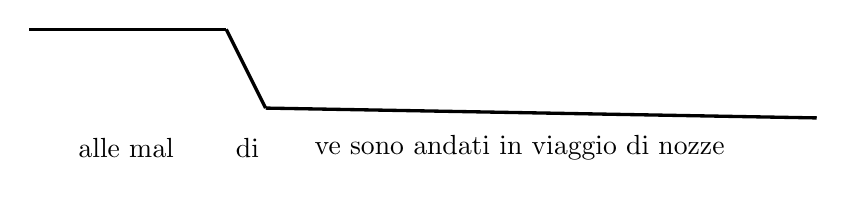
\begin{tikzpicture}[yscale = 0.5]
			
			\draw [very thick] (0,2.5) -- (2.5,2.5);
			\draw [very thick] (2.5,2.5) -- (3,0.5);
			\draw [very thick] (3,0.5) -- (10,0.25);
			
			\node[anchor=west] at (0.5,-0.5) {alle mal};
			\node[anchor=west] at (2.5,-0.5) {di};
			\node[anchor=west] at (3.5,-0.5) {ve sono andati in viaggio di nozze};
		\end{tikzpicture}

	\caption[Mirative fronting \textit{$_F$Alle Maldive$_F$ sono andati in 
	viaggio di nozze!}]{Mirative fronting \textit{$_F$Alle Maldive$_F$ sono andati in viaggio di nozze!} `They went $_F$to the Maldives$_F$ on honeymoon!' \citep{BianchiBocciCruschina.2016}.}\label{fig:mirative_fronting_MALEDIVE}
\end{figure}

\begin{figure}

		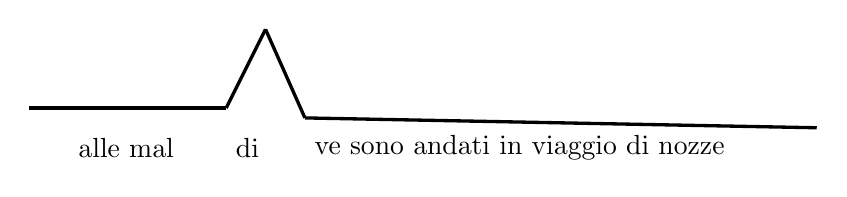
\begin{tikzpicture}[yscale = 0.5]
			
			\draw [very thick] (0,0.5) -- (2.5,0.5);
			\draw [very thick] (2.5,0.5) -- (3,2.5);
			\draw [very thick] (3,2.5) -- (3.5,0.25);	
			\draw [very thick] (3.5,0.25) -- (10,0);
			
			\node[anchor=west] at (0.5,-0.5) {alle mal};
			\node[anchor=west] at (2.5,-0.5) {di};
			\node[anchor=west] at (3.5,-0.5) {ve sono andati in viaggio di nozze};
		\end{tikzpicture}

	\caption[Contrastive fronting \textit{$_F$Alle Maldive$_F$ sono andati in viaggio di nozze!}]{Contrastive fronting \textit{$_F$Alle 
			Maldive$_F$ sono andati in viaggio di nozze!} `They went $_F$to the Maldives$_F$ on honeymoon!' 
		\citep{BianchiBocciCruschina.2016}.}\label{fig:contrastive_fronting_MALEDIVE}
\end{figure}



%\begin{figure}[H]
%	\includegraphics[width=.92\linewidth]{gfx/figure_contrastive_fronting_ALLE_MALEDIVE_2.png}
%	\caption[Contrastive fronting \textit{$_F$Alle Maldive$_F$ sono andati in viaggio di nozze!}]{Contrastive fronting \textit{$_F$Alle 
%			Maldive$_F$ sono andati in viaggio di nozze!} `They went $_F$to the Maldives$_F$ on honeymoon!' 
%		\citep{BianchiBocciCruschina.2016}.}\label{fig:contrastive_fronting_MALEDIVE}
%\end{figure}

\citet[5]{BianchiBocciCruschina.2016} argue that corrective readings for fronting are available in assertions functioning as a partial denial of a previous assertion (\ref{ex:correctivefrontingITALIANassertion}), whereas they are not available in questions functioning as a partial correction of a previous question (\ref{ex:correctivefrontingITALIANquestion}). This is valid for Italian, but also for Spanish. Whereas fronting in Spanish has long been described as exclusively linked to focus marking in corrective contexts, \citet{Cruschina.2019} shows that speakers also accept fronting in mirative contexts. In fact, fronting receives significantly higher acceptability scores in mirative all-new contexts than in corrective reactions to previous assertions.

\begin{exe}
\ex\label{ex:correctivefrontingITALIANassertion} Italian
\begin{xlist}[A:]
	\exi{A:}[]{Gianni ha regalato una collana a Maria. 
	\glt `John gave a necklace to Maria.'}
	
	\exi{B:}[]{No. \textit{Un anello} le ha regalato.
	\glt `No. A \textit{ring} (is what) he gave her.' }
\end{xlist}
\ex\label{ex:correctivefrontingITALIANquestion} 
\begin{xlist}[A:]
	\exi{A:}[]{La domanda cruciale è: ha insultato il suo collega?
	\glt `The crucial question is: did he insult his colleague?'}
	\exi{B:}[\#]{\textit{Il direttore} ha insultato?
	\glt `(Is it) \textit{the director} (whom) he insulted?'}
\end{xlist}
\end{exe}

Examples such as (\ref{ex:mirativefrontingCRUSCHINA}) have occasionally been acknowledged in the literature on the syntax and intonation of Spanish 
\citep{Reich.2018,Leonetti.2009}. But the main insight they provide has 
yet to penetrate research on the syntax-prosody interface in general, 
namely that at-issue meaning and \ac{NAI} meaning can be encoded via 
different channels and should be tested for independently.


\begin{exe} 
	\ex  \citet[131]{Cruschina.2019}\label{ex:mirativefrontingCRUSCHINA}\\
	¡Y yo que pensaba que no tenían ni un euro! ¡¿Sabes qué?! \\
	¡\textit{A las MalDIvas} fueron de luna de miel!
	\glt `I thought they were penniless! Guess what?! To the Maldives they went on honeymoon!'
\end{exe}

The analysis provided by \citet{BianchiBocciCruschina.2016} for mirative fronting differs from the analysis for \textit{wh}-exclamatives in \citet{ZanuttiniPortner2003} in three ways. Firstly, the at-issue content of declaratives with mirative fronting is asserted, instead of being presupposed to be true. In this sense, the root sentence resembles an ordinary statement. Secondly, the fronted constituent triggers a set of alternatives, both in corrective and in mirative contexts. Thirdly, the prosodically marked case of fronting conventionally implicates that ``the proposition expressed by the clause is less likely than at least one distinct alternative proposition with respect to a contextually relevant modal base and stereotypical ordering 
source.'' \citep[13]{BianchiBocciCruschina.2016} 

I briefly recapitulate some of the definitions necessary for an understanding of this approach based on \citet[30--43]{Kratzer.2012} and \citet[50--85]{Portner.2009}. Modal logic starts from a set of atomic sentences $\{p, q, r, \ldots\}$ and the logical relations Negation ($\neg \alpha$), Conjunction ($\alpha \wedge \beta$), Disjunction ($\alpha \vee \beta$), and Possibility ($\Diamond\alpha$). Possible worlds semantics further assumes a set of possible worlds \textit{W} conceivable by humans, e.g. \{\textit{u}, \textit{v}, \textit{w}, \textit{x}, \textit{y}, \textit{z}\}.%\footnote{Material Implication ($\alpha \rightarrow \beta$) and Necessity ($\Box\alpha$) can be derived from them \citep[13]{Portner.2009}: $\alpha \rightarrow \beta = \neg \alpha \vee \beta$; $\Box\alpha = \neg\Diamond\neg\alpha$.}

A proposition $p$ is the set of those possible worlds in which it is true. This is the case for $w \in W \text{ iff } w \in p$. Modal forms are taken to invoke a conversational background \textit{f}, in the light of which they are interpreted. We could rephrase (\ref{ex:mirativefrontingCRUSCHINA}) as `\textit{In view of what I know}, it is to the Maldives that they went on honeymoon!', which would be an epistemic \textit{modal base}. So a conversational background contributes premises for drawing conclusions about what is the state of affairs. In a context \textit{c} containing a speaker \textit{a} and for a world \textit{w} and a domain \textit{D} in which \textit{a} exists, a conversational background is formalized as a function \textit{f}(\textit{w}) $=$ \{\textit{p} : \textit{a} knows/sees/\ldots $p$ in \textit{w}\}. The set obtained serves as a \textit{modal base}. A non-exhaustive list of types of conversational backgrounds are listed in (\ref{ex:conversationalbackgrounds}).
	
\begin{exe}
\ex\label{ex:conversationalbackgrounds}
\begin{xlist}
	\ex Epistemic: \textit{f}(\textit{w}) is a set of facts known in \textit{w}.
	\ex Stereotypical: \textit{f}(\textit{w}) is a set of expectations about \textit{w}.
	\ex Teleological: \textit{f}(\textit{w}) is a set of goals in \textit{w}.
	\ex Bouletic: \textit{f}(\textit{w}) is a set of desires in \textit{w}.
	\ex Deontic: \textit{f}(\textit{w}) is a set of rules in force in \textit{w}.
\end{xlist}
\end{exe}

A crucial task of modal reasoning is to establish accessibility relations between possible worlds. Since propositions are sets of possible worlds, conversational backgrounds are sets of sets of worlds. To establish accessibility relations, it is more convenient to work with the set of worlds in which all $p$ in \textit{f}(\textit{w}) are true, which is the intersection $\cap f(w)$. A world \textit{v} is accessible from \textit{w} in an epistemic conversational background \textit{f} iff $\cap f(w) \subseteq v$ (if every fact known by the speaker in \textit{w} is true in \textit{v}). An epistemically accessible world in this sense is someone's truth or belief space. A world \textit{v} is accessible from \textit{w} in a deontic conversational background \textit{f} iff $\cap f(w)\subseteq v$ (if every rule in force in \textit{w} is true in \textit{v}). A deontically accessible world in this sense is a state of order. 

The strength or force of the conclusions drawn under the premises established by the modal base is determined by a second modal relation (a set of propositions A called the \textit{ordering source}), which can be based on a different conversational background. It is formalized as a function \textit{g}(\textit{W}) which gives a subset of the power set of W ($A \subseteq \text{Pot}(W)$) and serves to induce a partial ordering $\leq_A$ on W.\footnote{See also \citet[644]{Kratzer.1991} and \citet[64]{Portner.2009} on how two worlds \textit{v} and \textit{w} in \textit{W} can be ordered according to how many propositions in A (e.g. $\{p,q,r\}$) are true (e.g. just one, $\{p\}, \{q\}, \{r\}$, or two, $\{p,q\}, \{p,r\}, \{q,r\}$, or three, $\{p,q,r\}$). In short, they are partially ordered by ranking the cardinalities of the subsets of the power set of \textit{W}. Note that $\text{Pot}(W)$ is just a different form of writing $\mathfrak{P}(W)$.}

Coming back to the proposal by \citet{BianchiBocciCruschina.2016}, we should note that the mirative import consists in evaluating possible worlds as less expectable than another proposition obtained with an alternative focus value given two conversational backgrounds, which are the circumstances of conversation (modal base) and knowledge about the normal course of events (ordering source). We could again rephrase (\ref{ex:mirativefrontingCRUSCHINA}) as `\textit{In view of what I know}, it is to the Maldives that they went on honeymoon. \textit{In view of what I expect}, the set of propositions that are true in such a world is smaller than the set of propositions true in a different accessible world.' Note that this specific implementation of mirativity is different from similar proposals by \citet{Grosz.2012} in not requiring any contextually given likelihood threshold, which is intended to allow for out-of-the-blue miratives in which the only requirement is the possibility to come up with some more likely alternative.

At this point, it is important to stress the difference between surprise and mirativity. Surprise is often counted as one of the primary emotions which are recognized across cultures. It is typically caused by the violation of an expectation and results in a state of arousal that becomes visible in a specific and universal facial expression. Boredom has been proposed as the psychological counterpart to surprise \citep[139, 406, 831, 1053]{VandenBos.2015}.
 
Mirativity, on the other hand, takes on different forms and ways of expression in the languages of the world.\footnote{See \citet{DeLancey.2012} for an overview of the morphological means of encoding mirativity, and \citet{DiewaldSmirnova.2010} for why non-morphological ways of encoding meanings such as mirativity should be analyzed in much the same fashion (pace \cite{Aikhenvald.2012}).} It can be expressed without a state of arousal, since it is, like all pragmatic meanings, a public discourse commitment \citep{FarkasBruce.2010} that not necessarily expresses the speakers  true internal state. A mirative can be a lie, surprise cannot. It can also refer to the violation of the hearer's expectations \citep{HengeveldOlbertz.2012,RettSturman.2020}.\footnote{Note that a study on the features associated with nouns for surprise in a number of languages found a strong positive association with novelty, but not with power, arousal, or valence \citep{FontaineSchererSoriano.2013}.} And since it is not necessarily linked to arousal, it need not be accompanied by facial expressions and can be communicated without any visual cue (e.g. on the phone).\footnote{Cognitive processing of non-emotional abstract categories such as mirativity may, however, involve neuronal circuits reaching from multi-modal cortical areas into face-related sensorimotor areas \citep{DreyerPulvermueller.2018}. See \citet{XiangKuperberg.2014} on the neuronal effects of reversing expectations during discourse comprehension.} We should therefore distinguish between surprise and mirativity, which is the relation between expectations and asserted beliefs.\footnote{A recent in-depth discussion of surprise and mirativity can be found in \citet[35--77]{Kraus.2018}. After having meticulously reviewed possibilities of modeling surprise, she concludes that calculating either a threshold or a degree for surprise is not crucial to the linguistic phenomena she investigates (German and English modal particles and intonational patterns, \citealt[53]{Kraus.2018}). This is to be expected if mirativity does not depend on a feeling of surprise, but rather on communicative intentions.} \citet[16]{BianchiBocciCruschina.2016} also report on cases in which prosodically marked fronting takes on a value of discontent. These cases are prosodically similar to mirative fronting, which is unproblematic given that they are also semantically similar. The main difference is that they are evaluated according to a bouletic ordering source, rather than a stereotypical one.

From the point of view of a decompositional approach to Spanish 
intonation, there is therefore an empirical and a theoretical question to be answered. The empirical question is if the mirative import present in prosodically marked cases of fronting is also available in other syntactic contexts. Coming back to the types of statements presented in \autoref{tab:intonationalcategoriesPRIETOsmall}, we need to check if 
\textit{wh}-exclamatives differ systematically from declaratives in terms of their intonation. If this is not the case, I expect there to be the following prosodic minimal pairs: $\pm$mirative \textit{wh}-exclamatives and $\pm$mirative declaratives.\footnote{\citet{Rett.2011} can be credited with first acknowledging the possibility of a mirative import in both \textit{wh}-exclamatives and ``intonation only'' exclamatives. Yet she does not acknowledge the possibility of non-mirative \textit{wh}-exclamative, which blurs the contribution of intonation.} The theoretical question is about the status of mirative import relative to other prosodically expressed meanings that distinguish sentence types (declarative, interrogative, \ldots) or mark the corroboration of expectations (obviousness), rather than their violation. In \sectref{ch:3.2}, I discuss the relation between these two concepts as it shows in work on intonation. This discussion highlights the need for a formal model integrating different aspects of discourse meaning (modalized at-issue and non-at-issue commitments in combination with relative polarity), which is laid out in \sectref{ch:3.3}.



\section{Decomposing statements of the obvious}
\label{ch:3.2}

As already mentioned in \chapref{ch:2}, accounts of Spanish intonation often include statements of the obvious. \citet{BeckmanETAL.2002} describe a redundancy contour consisting of two rises and a facultative fall.\footnote{A contour difficult to translate into current ToBI conventions, given that the first rise seems to not be part of the nuclear configuration and the second rise could be either L+H* L\% or L* HL\% (\autoref{fig:redundancycontourSPANISH}).} \citet[277]{EstebasVilaplanaPrieto.2008}, \citet{EstebasVilaplanaPrieto.2010}, \citet{Prieto2009-2013}, and \citet{HualdePrieto2015} all mention the L+H*L!H\% contour, which has also been found in insubordinates by \citet{ElviraGarcia.2016}. A second contour often found in insubordinates is L* HL\%. Different accounts of the semantic contribution of this contour can be found in the literature. It is either seen as ``foco contrastivo con matiz de obviedad'' `contrastive focus with obvious nuance' \citep[277]{EstebasVilaplanaPrieto.2008}, as an emphatic contradiction \citep[369]{HualdePrieto2015}, or simply as a statement of the obvious \citep{TorreiraGrice.2018}. 

%If we take expectability to be the only relevant level of meaning here, obviousness could be seen as the antonym of a mirative statement \citep{Reich.2018}. Instead of violating expectations, a statement of the obvious would corroborate expectations about a proposition. Yet proposals for distinguishing between obviousness and counterexpectational nuances by means of intonation in Spanish suggest that they can sound very much alike.
Regarding the L+H* L!H\% contour, there is a debate about the effect of timing and scaling that touches at the heart of the question about whether obviousness and mirativity are encoded phonologically or phonetically. \citet[278]{Hualde.2014} proposes that an utterance with an L+H* L!H\% contour can be turned from a statement of the obvious into an incredulous surprise simply by increasing duration and pitch excursion. Figures~\ref{fig:exclamation_HUALDE} and~\ref{fig:exclamation_HUALDE_PRIETO_surprise_obvious}, both produced by Hualde himself, are intended to illustrate this difference.

\begin{figure}
		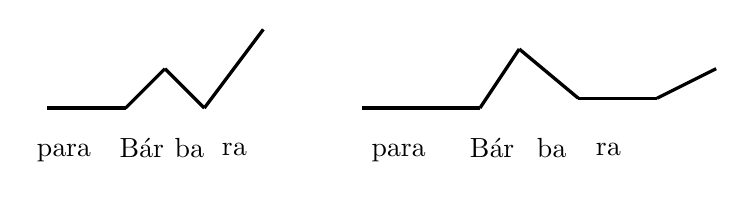
\begin{tikzpicture}[yscale = 0.5]
			
			\draw [very thick] (0,0) -- (1,0);
			\draw [very thick] (1,0) -- (1.5,1);
			\draw [very thick] (1.5,1) -- (2,0);
			\draw [very thick] (2,0) -- (2.75,2);
			
			
			\draw [very thick] (4,0) -- (5.5,0);
			\draw [very thick] (5.5,0) -- (6,1.5);
			\draw [very thick] (6,1.5) -- (6.75,0.25);
			\draw [very thick] (6.75,0.25) -- (7.75,0.25);
			\draw [very thick] (7.75,0.25) -- (8.5,1);
			
			\node[anchor=west] at (-0.25,-1.15) {para};
			\node[anchor=west] at (0.8,-1) {Bár};
			\node[anchor=west] at (1.5,-1) {ba};
			\node[anchor=west] at (2.1,-1.05) {ra};

			\node[anchor=west] at (4,-1.15) {para};
			\node[anchor=west] at (5.25,-1) {Bár};
			\node[anchor=west] at (6.1,-1) {ba};
			\node[anchor=west] at (6.85,-1.05) {ra};

		\end{tikzpicture}
	\caption[Obviousness and surprise-echo intonation on \textit{Bárbara}]{Obviousness (left) and ``surprise-echo'' (right) intonation on 
	\textit{Bárbara} \citep[278]{Hualde.2014}.}\label{fig:exclamation_HUALDE}
\end{figure}

\begin{figure}
		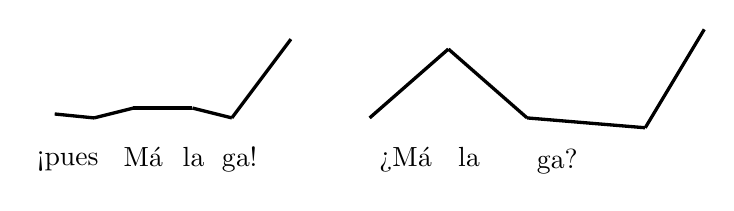
\begin{tikzpicture}[yscale = 0.5]
			
			\draw [very thick] (0,0.1) -- (0.5,0);
			\draw [very thick] (0.5,0) -- (1,0.25);
			\draw [very thick] (1,0.25) -- (1.75,0.25);
			\draw [very thick] (1.75,0.25) -- (2.25,0);
			\draw [very thick] (2.25,0) -- (3,2);			
			
			\draw [very thick] (4,0) -- (5,1.75);
			\draw [very thick] (5,1.75) -- (6,0);
			\draw [very thick] (6,0) -- (7.5,-0.25);
			\draw [very thick] (7.5,-0.25) -- (8.25,2.25);
			
			\node[anchor=west] at (-0.35,-1.1) {¡pues};
			\node[anchor=west] at (0.75,-1) {Má};
			\node[anchor=west] at (1.5,-1) {la};
			\node[anchor=west] at (2,-1.05) {ga!};
			
			\node[anchor=west] at (4,-1.05) {¿Má};
			\node[anchor=west] at (5,-1) {la};
			\node[anchor=west] at (6,-1.1) {ga?};
			
		\end{tikzpicture}
	\caption[Obviousness and surprise-echo intonation on \textit{Málaga}]{Obviousness 
	(left) and ``surprise-echo'' (right) intonation on 
	\textit{Málaga} \citep[379]{HualdePrieto2015}.}\label{fig:exclamation_HUALDE_PRIETO_surprise_obvious}
\end{figure}


%\begin{figure}
%	\centering
%	
%	\includegraphics[width=0.92\linewidth]{gfx/figure_exclamation_HUALDE.png}
%	\caption[Obviousness and surprise-echo intonation on \textit{Bárbara}]{Obviousness (left) and ``surprise-echo'' (right) intonation on 
%	\textit{Bárbara} \citep[278]{Hualde.2014}.}
%	\label{fig:exclamation_HUALDE}
%
%\bigskip
%
%\hspace*{-0.4cm}
%	\includegraphics[width=.92\linewidth]{gfx/figure_surprise_obviousness_MALAGA.jpg}
%	\caption[Obviousness and surprise-echo intonation on \textit{Málaga}]{Obviousness 
%	(left) and ``surprise-echo'' (right) intonation on 
%	\textit{Málaga} \citep[379]{HualdePrieto2015}.}\label{fig:exclamation_HUALDE_PRIETO_surprise_obvious}
%\end{figure}

What observations about these examples are possible from visual inspection? Firstly, the presence of a final rise seems similar to so-called rising declaratives, yet the status of rising declaratives as either declaratives, interrogatives, or exclamatives remains unclear (note the change between exclamation marks and question marks, which indicates the uncertainty about an appropriate classification). Secondly, the scaling of the final rise seems inconsistent. While in \autoref{fig:exclamation_HUALDE} there is clearly a higher final rise in the condition described as obvious than in the one described as ``echo-surprise'', in \autoref{fig:exclamation_HUALDE_PRIETO_surprise_obvious} the opposite seems to be the case. This is important because scaling is phonologically included as downstep in the L+H*L!H\% transcription. Thirdly, the target word in the surprise condition 
is lengthened by approx. 20ms, mostly due to the duration of the final 
syllable. Finally, the obvious condition is further disambiguated by an initial 
particle \textit{pues} `well' with falling intonation. This coincides with 
the data in \citet{Prieto2009-2013}, in which 17 out of 23 statements of the obvious from different Spanish varieties show initial particles
(\textit{pues} or a particle such as \textit{hombre} or \textit{mujer}).\footnote{Particles seem to be present in many utterances with marked intonation. We come back to this topic in \sectref{ch:3.3} and \sectref{ch:5.1}.}



%\noindent\begin{minipage}{\textwidth}
%	\bigskip
%	\begin{exe}
%		\begin{spacing}{0.6}
%			\ex\label{ex:surpriseobviousPRIETOROSEANO} Transcription of 
%			\autoref{fig:exclamativePRIETOROSEANO} and 
%			\autoref{fig:obviousstatementPRIETOROSEANO}
%			
%			\begin{xlist} 
%				\ex 
%				{[}\begin{IPA}"be.Be.li.mo."na.Da\end{IPA}\hspace*{.74cm}{]}\\
%				{[}L+<H* \hspace*{.3cm} L+H* L!H\%{]}\\
%				‘\textit{I'm drinking lemonade! (of course)}’ \\
%				\ex 
%				{[}\begin{IPA}"ke.o."loR.a.pan.tan."bwe.no\end{IPA}\hspace*{.2cm}{]}\\
%				{[}\hspace*{.22cm} L+H* \hspace*{1.47cm} L+¡H* L\%{]}\\
%				‘\textit{What a good smell of bread!}’ \\
%			\end{xlist}
%		\end{spacing}
%	\end{exe}
%\end{minipage}

From a theoretical point of view, the main problem is the claim that the difference between exclamative and obvious intonation lies solely in timing and scaling differences.
This contrasts sharply with the proposal in \autoref{tab:intonationalcategoriesPRIETOsmall}, where exclamatives are listed with L+¡H* L\% and therefore lack a final rise. If we assume that obviousness and mirativity are incompatible meanings \citep{Reich.2018}, an intonational similarity between the two would mean that listeners would need to perceive quite subtle cues in order to distinguish between them. An alternative interpretation would be that both Figures~\ref{fig:exclamation_HUALDE} and~\ref{fig:exclamation_HUALDE_PRIETO_surprise_obvious} are obviousness contours, but anchored to different kinds of expectations. According to a proposal put forward for the so-called Surprise Redundancy Contour in English \citep[497]{SagLiberman.1975}, the nuance of surprised obviousness ``could arise because the intonation of this utterance is expressing surprise at the very fact that it's necessary for the speaker to be asking such a question at all.'' So instead of evaluating a proposition as unexpected, such an utterance would mark it as so highly expectable as to render any inquiry about it a surprise. This kind of discourse-level surprise would fit in with the idea of redundancy also captured in the notion of ``counterexpectational echo question'' \citep[379]{HualdePrieto2015}.

If we accept such an interpretation, it poses an even greater challenge for the formal treatment of intonational meaning. How can we capture the difference between a modal evaluation of a state of affairs (as expressed in a proposition) and the evaluation of a prior speech act? How can we distinguish between these two very different layers of meaning? In \sectref{ch:3.3.1}, I propose to tackle this problem by asking for every example a set of very basic question: Is this sentence a provocation or a response? If it is a response, is the provocation an assertion or a (biased) question? What is the current Question Under Discussion (QUD)? What are the propositions that interlocutors have publicly committed to? Are there points of (dis)agreement? What would be a marked or unmarked response? More generally, I want to stress that intonation research needs to start from the assumption of a \textit{Provocation-Response Nexus} in which even minor prosodic or syntactic differences in the provocation may lead to intonational differences in responses. Therefore, investigation of sentence-level prosody in responses is close to impossible without a detailed knowledge of the lexical, syntactic, and prosodic form of the respective provocation.

Research on intonation has only recently started to make provocations maximally explicit. Examples for statements of the obvious make this particularly clear. To start with the L+H*L!H\%, see the example \autoref{fig:obviousstatementAIEE} and the respective context in (\ref{ex:simujerdeguillermo}) \citep{PrietoRoseano2009encuestacastilia}.\footnote{The mid-tone M was later replaced by !H \citep[362]{HualdePrieto2015}.}

\begin{exe}
	\ex\label{ex:simujerdeguillermo} Context for \autoref{fig:obviousstatementAIEE} \\
	Estás con una amiga y le cuentas que María, una amiga común, está embarazada. Ella te pregunta que de quién está embarazada y tú te extrañas mucho de que no lo sepa porque todo el mundo sabe que es de Guillermo, su novio de toda la vida. ¿Qué le dices? 
	\glt ‘You're with a friend and you tell her that María, a mutual friend, is pregnant. She asks you who she is pregnant by and you're astonished that she doesn't know because everybody knows that it's by Guillermo, her life-long boyfriend. What do you tell her?’ 
\end{exe}



\begin{figure}
\includegraphics[width=.95\linewidth]{gfx/figure_statement_of_the_ovbious_AIEE_new_2.png}
\caption[Obvious declarative \textit{¡Sí, mujer, de Guillermo!}]{Statement of the 
	obvious \textit{¡Sí, mujer, de Guillermo!} `Yes, woman, by Guillermo!' 
	\citep{Prieto2009-2013}. Response to \textit{¿De quién está embarazada?} 
	`Who is she pregnant by?' \citep{PrietoRoseano2009encuestacastilia}, 
	probably reinterpreted as response to a biased \textit{¿Está embarazada de 
		Guillermo?} `Is she pregnant by 
	Guillermo?'.  \href{http://prosodia.upf.edu/atlasentonacion/enquestes/espanol/madrid/frases/mp3/10.mp3}{\faVolumeUp} \href{http://prosodia.upf.edu/atlasentonacion/enquestes/espanol/madrid/index.html}{\faExternalLink*}} \label{fig:obviousstatementAIEE}
\bigskip
\end{figure}

The provocation in (\ref{ex:simujerdeguillermo}) does not seem congruent with the answer \textit{¡Sí, mujer, de Guillermo!}. If the provocation had actually been the unbiased \textit{wh}-question \textit{¿De quién está embarazada?}, neither the polarity particle \textit{sí} nor the particle/vocative use of \textit{mujer} would have been warranted. Either the experimenters gave a provocation such as \textit{Está embarazada de Guillermo, ¿verdad?} `She's pregnant by Guillermo, right?', or the participant interpreted the context description in such a way.

A similar case in point is \autoref{fig:paraquemeriendeLHLHfigure}, partially repeated for convenience in \autoref{fig:paraquemeriendeLHLHfigurerepeat}. The context, repeated in (\ref{ex:paraquemeriendeLHLHrepeat}), does not provide the exact form of the provocation, but we can assume it to be an imperative, perhaps in combination with an explanation of the sort \textit{Por favor, ¡lleva Marina a la carnicería! Tú sabes por qué te lo pido.} `Please, take Marina to the butcher's. You know why I'm asking you about it.' Given that the \textit{Discourse Completion Task} methodology \citep{VanrellFeldhausenAstruc.2018} standardly requires the experimenter to pre-construct a written context but leaves any possible verbal provocation open for the experimenter to deliver \textit{ad-hoc}, we do not know the exact form of the provocation. It may also be the case that the experimenter provided the contexts without uttering a provocation. In this case, I would argue that the participants still need to imagine a provocation in order to choose an appropriate response.

\begin{exe}
\ex \label{ex:paraquemeriendeLHLHrepeat}  Context for \autoref{fig:paraquemeriendeLHLHfigurerepeat}\\
	CONTEXTO: Tú sabes que siempre que llevo a Lorena a la carnicería se compra médula para merendar y a ti no te gusta ir a la carnicería pero piensas que si es por la médula de Marina te tendrás que sacrificar.\\
	ENTREVISTADORA: Yo te digo que lleves a Marina [sic!] a la carnicería y tú me respondes:\\
	RESPUESTA: ¡Sí, hombre! Para que meriende.
	\glt `CONTEXT: You know that I always take Lorena to the butcher's [for her to] buy herself some meat-soup for lunch and you don't like going there but think that when it comes to Marina's meat-soup you need to make that sacrifice.' \\
	`INTERVIEWER: I tell you to take Marina to the butcher's and you answer me:' \\
	`RESPONSE:	¡Sure, man! For her to have lunch.'
\end{exe}


\begin{figure}
	\includegraphics[width=.95\linewidth]{gfx/figure_si_hombre_por_que_REPEAT_ELVIRA_GARCIA.png}
	\caption[\textit{¡Sí, hombre! Para que meriende.}]{\textit{¡Sí, hombre! Para que meriende.} `Sure, man! For her to have lunch.' \citep{ElviraGarcia.2016}.}\label{fig:paraquemeriendeLHLHfigurerepeat}
\end{figure}

Turning to examples of the L* HL\% contour, the difficulty of determining the nature of a particular \textit{Provocation-Response Nexus} becomes apparent. In (\ref{ex:comosiVsubREPEAT}), the highly complex declarative/imperative provocation can be split up into several assertions and presuppositions, only one of them (she eats meat-soup) being challenged by the response.

\begin{exe}
	\ex  \label{ex:comosiVsubREPEAT} Context for \autoref{fig:comosiVsubFIGURE189} (page \pageref{fig:comosiVsubFIGURE189})\\
	CONTEXTO: Imagina que soy tu canguro y la de tu hermana. Tú quieres pasar
	una temporada sin merendar para adelgazar y yo no te dejo y te digo...\\
	ENTREVISTADORA: Mira, tu hermana está delgada y sin dejar de tomar ninguna comida \\
	CONTEXTO: Pero tú sabes que ella no merienda (lo tira a la basura), y me respondes:... \\
	RESPUESTA: ¡Como si merendara médula!
	\glt `CONTEXT: Imagine that I'm the nanny of you and of your sister. You want to skip lunch for a while to lose weight, but I don't let you and tell you...'\\
    `INTERVIEWER: Look your sister is thin without skipping meals' \\
    `CONTEXT: But you know that she doesn't have lunch (she throws it away), and you answer me...' \\
	`RESPONSE: ¡As if she'd be having meat-soup for lunch!'
\end{exe}

A clearer case of obvious stimulus is (\ref{ex:perosiVX}), repeated in (\ref{ex:perosiVX2}) for convenience. Here, the \textit{todos los días} `every day' stimulus, presented by the experimenter herself, stands in contrast with the assertion by the experimenter and forces the participant to disagree based on mutually shared knowledge.

\begin{exe}
	\ex  \label{ex:perosiVX2}  CONTEXTO: Sabes que Marina merienda todos los días verdura. \\
	ENTREVISTADORA: Marina meriende chocolate. \\
	RESPUESTA: 	
	\begin{xlist}
		\ex ¡Pero si merienda \textbf{mé}dula! (antepenultimate) 
		\ex ¡Pero si merienda ver\textbf{du}ra! (penultimate) 
		\ex ¡Pero si merienda guara\textbf{ná}! (ultimate, $-$coda)
		\ex ¡Pero si merienda bibe\textbf{rón}! (ultimate, $+$coda)  
	\end{xlist}
	
	\glt `CONTEXT: You know that Marina is having vegetables for lunch every day.' \\
	`INTERVIEWER: Marina having chocolate for lunch.' \\
	`RESPONSE:' 
	\begin{xlist}
		\ex `¡But SI she is having meat soup for lunch!' 
		\ex `¡But SI she is having vegetables for lunch!' 
		\ex `¡But SI she is having guaraná for lunch!' 
		\ex `¡But SI she is having a baby bottle for lunch!' 
	\end{xlist}
\end{exe}

\begin{figure}
	\includegraphics[width=\linewidth]{gfx/figure_como_si_187_ELVIRA_GARCIA_new.png}
	\caption{\textit{¡Como si merendara médula!} `As if she'd be having meat-soup for lunch!' 
		\citep[187]{ElviraGarcia.2016}.}\label{fig:comosiVsubFIGURE189}
\end{figure}

\largerpage Corpus examples require a close reading of the context in order to capture their intricate discourse relations. (\ref{ex:claroesquedeesoTORREIRAGRICE}), repeated here as (\ref{ex:claroesquedeesoTORREIRAGRICErepeat}), is presented by \citet{TorreiraGrice.2018} as an obvious assertion. Yet the dynamics of interaction seem more complex. In (\ref{ex:claroesquedeesoTORREIRAGRICErepeat}a), 2RM asserts that equal treatment is required in school for boys and girls. In (\ref{ex:claroesquedeesoTORREIRAGRICErepeat}b), 2CM accepts this, but restricts the acceptance to the level of education. 2RM accepts this restriction in (\ref{ex:claroesquedeesoTORREIRAGRICErepeat}c). Nevertheless, 2CM explains the restriction in (\ref{ex:claroesquedeesoTORREIRAGRICErepeat}d) as if there had been no agreement in (\ref{ex:claroesquedeesoTORREIRAGRICErepeat}c). The reaction by 2RM in (\ref{ex:claroesquedeesoTORREIRAGRICErepeat}e) should be seen not only as a statement of the obvious, but one which rejects the necessity for clarification, given that the educational level was probably implied since the first mention of a school in (\ref{ex:claroesquedeesoTORREIRAGRICErepeat}a).

\begin{exe}
\ex\label{ex:claroesquedeesoTORREIRAGRICErepeat} NCCSp\_02\_3494
	\begin{xlist}
		\ex
		2RM: Pero en el colegio les tienes que tratar igual, o sea \ldots\\
		\hspace*{2em} `But in school you should treat them in the same way, I mean \ldots'
		\ex
		2CM: En nivel educa[tivo, que aprendan lo mismo].\\
		\hspace*{2em} `At the educational level, they should learn the same.'
		\ex
		2RM: \hspace{7em}[En educación, la educación,]\\
		\hspace*{9em} `In terms of education, education,'
		\ex
		2CM: Que aprendan lo mismo.\\
		\hspace*{2em} `They should learn the same.'
		\ex
		2RM: ¡\textbf{CLA}ro! \hspace{2em} ¡\textbf{Es} que \textbf{es} \textbf{e}so! \\
		\hspace*{3em} L* H(L\%) \\
		\hspace*{2em} `Of course! \hspace{1.5em} That's it!' \\
		\hspace*{2em} ¡\textbf{Es} que de \textbf{e}so se e\textbf{stá} ha\textbf{BLAN}do! ¡De educa\textbf{CIÓN}! \\
		\hspace*{2em} L* \hspace*{9.6em} H* L\% \hspace{4em} L* H(L)\% \\
		\hspace*{2em} `That's what's being discussed! \hspace{2.5em} Education!'
	\end{xlist}
\end{exe}

As with exclamatives and miratives, obviousness is too broad a label for different interactive stances. Saying that a sentence carries a nuance of surprise or obviousness is insufficient for determining the specific contribution of prosodic form to the discourse function of a turn in dialogue. Both corpus investigation and laboratory experiments need a deeper understanding of the interaction between different layers of discourse meaning. (Dis)agreement, discourse commitments, \ac{QUD} structure, and modal meaning need to be integrated when assigning a sentence-type to a prosodic form. In the following, I present a model that decomposes discourse functions, allowing us to be more precise about the meaning contribution of intonational markers.

\section{A model of meaning in dialogue}\label{ch:3.3}\largerpage[1.75]

\citet{FarkasBruce.2010} develop a model of meaning in dialogue to capture similarities and differences between assertive speech acts (such as declaratives) and inquisitive speech acts (such as polar interrogatives) in terms of the possible ways of reacting to them.{\interfootnotelinepenalty=10000\footnote{The term \textit{inquisitive} has since become much more central to semantic theory through the development of \textit{inquisitive semantics} \citep{CiardelliGroenendijkRoelofsen.2019}, a framework that will not be laid out in full detail here, though it should be compatible with what follows \citep{FarkasRoelofsen.2017}.}} It gives a formal account of their functions in dialogue and thereby provides the mechanisms necessary to predict markedness relations between different provocations and responses. It is essentially a dynamic model of the negotiation of \textit{Discourse Commitments} and the \textit{Question Under Discussion}. While the \ac{QUD} determines what is at-issue in a discourse context, Discourse Commitments are what links interlocutors to the \ac{QUD}. This combination has several advantages. It captures the intuition that dialogue can go wrong in different ways, either because interlocutors do not \textit{stick to the point} or because they cannot solve a disagreement. This focus on (dis)agreement is crucial to capture markedness relations between responsive speech acts that negotiate how interlocutors position themselves towards what is at-issue. Even more importantly for our current purpose, the model is also flexible enough to be expanded to non-at-issue meaning (\cite[89]{FarkasBruce.2010}, \cite{Rett.2021emotivemarkers,Rett.2021expressivesandmiratives}). After introducing the core model in \sectref{ch:3.3.1}, we show its limitations in dealing with the ambiguity of Spanish discourse markers in \sectref{ch:3.3.2}. We then include non-at-issue meanings in \sectref{ch:3.3.3} to capture their two levels of meaning: polar and modal.

\subsection{Reacting to assertions and polar questions}\label{ch:3.3.1}

According to \citet{Stalnaker.1974,Stalnaker.1978}, a declarative sentence 
is a conversational move made with the intention of adding its asserted 
content to the common background knowledge or \ac{CG} of the 
interlocutors. \citet{FarkasBruce.2010} stress the point that 
this move is only successful if no participant in the conversation 
objects. A declarative is therefore best understood as a proposal that 
triggers a process of several steps and choices. These steps have to do 
with different aspects of conversation that interlocutors keep track of, 
and the choices they make can be marked or unmarked. 

Firstly, interlocutors keep track of the current goal of the conversation. What sets questions and statements apart from imperatives and vocatives are their goals. Questions and statements inquire about the state of affairs, they participate in answering the current \ac{QUD} \citep{Roberts.2012,BeaverRobertsSimonsTonhauser.2017}. More generally, they attempt to capture the world in terms of words. Their direction of fit is words-to-world \citep{Searle1979}. Imperatives and vocatives, on the other hand, pursue goals in which the direction of fit is world-to-words. Both questions and statements can set a new goal by opening a new 
\ac{QUD}. \citet[86]{FarkasBruce.2010} christen the place-holder for the current
\ac{QUD} the \textit{Table}. It is a stack, to whose top items can be 
\textit{pushed}, from whose top items can be \textit{popped}, and from 
which an item can be \textit{removed}.\footnote{Push and pop are terms 
necessary to make reference to the top of a stack as opposed to an element 
of a set, which could simply be added or removed.} Conversational moves that put an issue on the \textit{Table} are called provocations, as opposed to responses which are defined by a requirement for a non-empty \textit{Table}. A second component of the \textit{\citeauthor{FarkasBruce.2010} Model} are \acp{DC} for each interlocutor. A declarative commits a speaker to $p$ by asserting it, but assertion and speaker commitment are not the same thing. Speakers can retract from a commitment that forms part of a set of commitments, whereas an assertion is an individual act of committing to the truth of a proposition. Unmarked moves add to the set of discourse commitments, removing a commitment is a marked move. This captures the relative ease with which many speech acts commit a speaker to a proposition, whereas removing a commitment requires explicit acknowledgment of an error or a lie. Markedness in terms of the model is therefore first and foremost semantic markedness. Yet, as we will see throughout, it fits neatly into a Greenbergian notion of markedness that links semantic complexity with overt coding, rare occurrence in texts, and neutralization in unmarked contexts \citep{Greenberg.1966}.\footnote{Pace \citet{Haspelmath.2006againstmarkedness}, I opt against reducing \textit{markedness} to \textit{frequency of use}, because frequency does not predict these relations to be universals (cross-linguistic and diachronic), which could be seen as the main point in \citet{Greenberg.1966} and \citet{FarkasBruce.2010}.}

\begin{sloppypar}
The conversational game proceeds in steps, each of which represents a 
\ac{K}. If both participants in a dialogue have publicly committed to a 
proposition, it is added to the \textit{cg}.\footnote{Note how the Stalnakarian notion of Common Ground becomes a derived component of the \acp{DC}. By convention, sets are in lowercase, so \ac{CG} is written \textit{cg} here.} Furthermore, a \ac{ps} keeps 
track of requirements imposed on upcoming moves by some types of 
sentences, among them assertions. By putting an item on the Table, a set of future Common Grounds is projected. In each of these Common Grounds the issue on the Table is decided. If there is just one \ac{CG} in $\ps$ (for example due to an assertion), \ac{K} is biased towards it.\footnote{Note, again, that the projected set is determined by the Tabletop.} This captures the idea that there are discourse contexts in which there are marked and unmarked ways for a dialogue to proceed. Notably, tacit agreement is built into the model.\footnote{While this insight has only recently been integrated into research on formal pragmatics, it is by no means a new idea that ``\textit{qui tacet, consentire videtur}'' `who is silent seems to consent' \citep[825]{BonifaceVIII.1584}.} An interlocutor can tacitly agree with an assertion, but (s)he cannot tacitly deny one. (\ref{ex:contextstate}) shows a graphic representation of a context state.
\end{sloppypar}

\begin{exe}
	\ex K: Context state \citep[89]{FarkasBruce.2010}.\label{ex:contextstate}\smallskip\\
		\begin{tabular}{|Z{6em}|Z{6em}|Z{6em}|Z{6em}|} \hline
			{A} & \multicolumn{2}{Z{12em}|}{{Table}} & {B} \\\hline
			DC$ _{a} $ & \multicolumn{2}{Z{12em}|}{S} & DC$_{b} $ \\ \hline
			\multicolumn{2}{|Z{12em}|}{Common Ground \textit{cg}} &
			\multicolumn{2}{Z{12em}|}{Projected Set $\ps$} \\ \hline
		\end{tabular}
\end{exe}

At the beginning of a dialogue K$_{1}$, the Table and the \acp{DC} are empty while the \textit{cg} already contains shared background knowledge 
(\ref{ex:contextstateINITIAL}). This assumption, innocent as it may seem, is actually one of the crucial differences between the \textit{Table} and standard \ac{QUD}-structure. For \citet[6:5]{Roberts.2012}, discourse starts with the \textit{Big Question} ``What is the way things are?''. Solving any sub-question of the \textit{Big Question} only brings interlocutors closer to this initial state, never to an empty \textit{Table}. In this sense, \citet{FarkasBruce.2010} take a micro-perspective within discourse, focusing on a smaller level of relevance in which issues are prototypically raised and solved (accepted or denied) in a window of one or two turns. Longer negotiations of one specific issue,\footnote{At the same level of specificity, not at the level of sub-questions.} while theoretically possible and empirically existent (see \chapref{ch:5}), become progressively more marked because they require successions of reversal and insistence.\footnote{Otherwise the issue is solved, either via tacit agreement or, as we will see below, an agreement to disagree.} It is this micro-perspective that allows for a model of the dynamics between adjacent turns, where it is highly important to track which interlocutor sets up an issue for discussion and which interlocutor denies it, accepts it, or evaluates it in other ways (see \sectref{ch:3.3.3}). I will call the status of a turn as either provocation or response its \textit{Turn Adjacency}, relating it to adjacent (directly previous or posterior) turns in terms of possible discourse anaphoric relations.\footnote{While purposefully close to the notion of adjacency pair in \citet{SchegloffSacks.1973} and \citet{SacksSchegloffJefferson.1974}, Turn Adjacency gears the perspective towards the different functions of the turns within such pairs with regard to Discourse Commitments.}

\begin{exe}
	\ex	K$_{1}$: Initial context state.\label{ex:contextstateINITIAL}\smallskip\\
		\begin{tabular}{|Z{6em}|Z{6em}|Z{6em}|Z{6em}|} \hline
			{A} & \multicolumn{2}{Z{12em}|}{{Table}} & {B} \\\hline
			 & \multicolumn{2}{Z{12em}|}{} &  \\ \hline
			\multicolumn{2}{|Z{12em}|}{Common Ground \textit{s$_1$}} &
			\multicolumn{2}{Z{12em}|}{Projected Set \textit{ps$_1$} $ = $ 
			$ \{$\textit{s$_1$}$\}$} \\ \hline
		\end{tabular}
\end{exe}

A declarative sentence is represented as a syntactic and prosodic form S[D].\footnote{The model remains agnostic about the representation of non-sentential turns with declarative prosody. Given that many non-sentential turns are responses that require sentential provocations, I will follow the \citeauthor{FarkasBruce.2010} formalism to keep the illustration as simple as possible.} Uttering a declarative denotes a declarative operator \textbf{D} (\ref{ex:declarativeoperator}).\footnote{Note that the original model by \citeauthor{FarkasBruce.2010} (\citeyear{FarkasBruce.2010}) coins an assertion operator \textbf{A} corresponding to S[D]. I follow \citet{Rett.2021emotivemarkers} in capturing the function of the declarative illocutionary mood under the operator \textbf{D} because I also attribute assertive force to sentences without declarative illocutionary mood which still upgrade doxastic discourse commitments (see \autoref{tab:biasedprovocations}); see also the notion of \textit{assertive family} in \citet[11--13]{Jary.2010} and  the relation between assertion and discursive commitment in \citet[157]{Brandom.19942001} and \citet[19--23]{Jary.2010}.} \citet[90]{FarkasBruce.2010} ``take it that a default assertion is performed when a participant X utters a declarative sentence \textit{S} with falling intonation.''\footnote{While they do not treat rising declaratives and tag-declaratives, they assume that they place specific demands on the input context.} \textbf{D} is a function that takes the sentence S[D], the speaker index a, and the input context state K$_{i}$ as arguments and gives an output context state K$_{o}$, in which the 
DC$_{a,o}$ is the union of \{\textit{p}\} and DC$_{a,i}$, T$_{o}$ is the result of \textit{pushing} $\{ p \}$ together with its sentence form S and the declarative sentential feature [D] on the input Table T$_{i}$, and the \ac{ps}$_{o}$ is the union of $\{ p \}$ and $\cg_i$ minus all the 
resulting inconsistent sets, which is represented by $\bar{\cup}$ and can 
be called \textit{consistent union}.\footnote{``Let $\ps= \{\cg_1, \ldots, \cg_n\}$ be a collection of sets of propositions (e.g. possible Common Grounds) and let $P = \{p_1, \ldots, p_m\}$ be a set of propositions. Then define \[\ps \bar{\cup} P = \{\cg_i \cup \{p_j\}| 1 \leq i \leq n, 1 \leq j \leq m\} - \{\cg' | \cg' \text{ is inconsistent}\}\] \citep[90]{FarkasBruce.2010}. I follow \citet{FarkasBruce.2010} in only listing the operation $\ps\bar{\cup}P$ in the formalization of the operators with no additional indications in the illustrations. At the risk of getting ahead of the discussion, I want to note here that canceling this consistency operation might be a side-effect of mirative provocations, since miratives proffer a proposition that is inconsistent with the \ac{CG} and therefore require interlocutors to re-evaluate the \ac{CG}.} The K$_{o}$ of \textit{A} over K$_{1}$ is K$_{2a}$, illustrated in (\ref{ex:contextstateSECOND}).

\begin{exe}
\ex\label{ex:declarativeoperator} \textbf{D} (S[D], a, K$_{i}$) = K$_{o}$ such that \hfill (all operators revised in \sectref{ch:3.3.2}) 
\begin{xlist}
	\ex $\DC_{a,o} = \DC_{a,i}\cup\{\textit{p}\}$ 
	\ex $T_{o} = \textit{push}(\langle S[D]; \{ p \} \rangle, T_{i})$
	\ex $\ps_{o} = \ps_{i}\bar{\cup}\{\textit{p}\}$ 
\end{xlist}

\ex	K$_{2a}$: A states `She drinks lemonade' relative to K$_{1}$
\label{ex:contextstateSECOND}\smallskip\\
\begin{tabular}{|Z{6em}|Z{6em}|Z{6em}|Z{6em}|} \hline
	A & \multicolumn{2}{Z{12em}|}{{Table}} & 
	B \\\hline
	\textit{p} & \multicolumn{2}{Z{12em}|}{$\langle $ `She drinks 
	lemonade'[D]; $ \{ p \} \rangle$} &  \\ \hline
	\multicolumn{2}{|Z{12em}|}{\textit{s$_2$}$=$ 
	\textit{s$_1$}} &
	\multicolumn{2}{Z{12em}|}{\textit{ps$_2$}$=$ 
	$\{$ s$_1$ $\cup $ $ \{$\textit{\textit{p}}$\}\}$} \\ \hline
\end{tabular}
\end{exe}

Once the Table is not empty, the conversation is driven by the 
need to empty it, or to settle the issue. A conversation is in a 
\textit{stable state} when the Table is empty. Conversational moves that 
place items on the Table bring with them a way of removing them by 
deciding upon them. This happens iff either $p$ or $\neg 
\textit{p}$ follows from \textit{cg}. Therefore, the most straightforward way of 
deciding upon an assertion is to confirm it. All other reactions to 
assertions are marked.

A polar question has as a syntactic\slash prosodic form S[I]. Given that \citet[94]{FarkasBruce.2010} are dealing with English, they take the syntactic form to be crucial. For Spanish, it would be a purely prosodic form L*~HH\% (\autoref{tab:intonationalcategoriesPRIETO}).\footnote{The low-rise contour has variously been transcribed as either L*~H\% or L*~HH\%. I use L*~HH\% here to acknowledge that scaling of final rises in polar questions seems to be higher than in other cases of final rises. See also \sectref{ch:6.3.4} on why further research is needed here.} Utte\-ring a polar question denotes a polar question operator \textbf{PQ} 
(\ref{ex:polarquestionoperator}). \textbf{PQ} is a function that takes the interrogative sentence
S[I] and the input context state K$_{i}$ as arguments and gives an 
output context state K$_{o}$, in which T$_{o}$ is the result of 
\textit{pushing} \{$\textit{p},\neg p$\} together with its sentence form S and the 
interrogative sentential feature [I] on the input Table T$_{i}$, and the 
\ac{ps}$_{o}$ is $ps_{i}$ with either
\{\textit{p}\} or \{$\neg p$\}. The K$_{o}$ of \textbf{PQ} over K$_{1}$ is 
K$_{2pq}$, illustrated in (\ref{ex:contextstateSECONDpq}). An important aspect of placing both S[I] and \{$\textit{p},\neg p$\} on the Table is the fact that S[I], though not asserted, is \textit{highlighted} and can serve as an antecedent for subsequent anaphoric expressions such as \textit{yes} and \textit{no} (\cite[254]{FarkasRoelofsen.2017} and references therein).

\begin{exe}
\ex\label{ex:polarquestionoperator} \textbf{PQ} (S[I], 
K$_{i}$) = K$_{o}$ such that 
\begin{xlist}
	\ex $T_{o} = \textit{push}(\langle S[I]; \{\textit{p},\neg 
	\textit{p}\}\rangle, T_{i})$
	\ex $\ps_{o} = \ps_{i}\bar{\cup}\{\textit{p},\neg 
	\textit{p}\}$ 
\end{xlist}

\ex	K$_{2pq}$: `Does she drink lemonade?' was asked relative to 
		K$_{1}$	\label{ex:contextstateSECONDpq}\smallskip\\
		\begin{tabular}{|Z{6em}|Z{6em}|Z{6em}|Z{6em}|} \hline
			A & \multicolumn{2}{Z{12em}|}{Table} & B \\\hline
			 & \multicolumn{2}{Z{12em}|}{$\langle$`She drinks 
				lemonade'[I]; $ \lbrace p,\neg p \rbrace\rangle$} &  \\ \hline
			\multicolumn{2}{|Z{12em}|}{\textit{s$_2$}$=$ 
				\textit{s$_1$}} &
			\multicolumn{2}{Z{12em}|}{\textit{ps$_2$}$=$ $\{$ s$_1$ $ \cup 
			$ $ \{$\textit{\textit{p}}$\}$, s$_1$ $ 
				\cup $ $ \{$\textit{$\neg p$}$\}$ $\}$} \\ \hline
		\end{tabular}
\end{exe}

As mentioned above, apart from \textit{initiating} questions and assertions, the model
provides a formalization of \textit{responding} conversational moves. Every response has a provocation, and the communicative effect of a responding move is conditioned by its provocation. Assertions and polar questions both place a proposition-de\-no\-ting sentence 
radical on the Table. Therefore, both allow for responses in terms of 
\textit{confirmation} and \textit{reversal}. The crucial difference 
between reactions to polar questions and assertions is that polar 
questions project their own reversal, whereas assertion reversal results in a \textit{conversational crisis}.

A conversation can be in three states: stable (no issue on the Table), 
unstable, and in crisis. A conversation is in crisis if either its 
\textit{cg} is inconsistent or all the sets in \ac{ps} are inconsistent 
(because the next \ac{K} would then have an inconsistent \textit{cg}). 
Denying an assertion creates a conversational crisis, because it 
commits the reacting interlocutor to a proposition that is incompatible 
with the current \ac{ps} and itself projects a \ac{ps} that is 
incompatible with a commitment already made. There are two solutions to a 
conversational crisis: retraction of a commitment by one of the 
interlocutors, or agreeing to disagree. What is important here is that 
neither of the two can happen tacitly. Either an interlocutor explicitly 
retracts from her incompatible commitment, or the two commitments remain 
in the respective \textit{DC}s without entering the Common Ground.

The \citeauthor{FarkasBruce.2010} model takes assertions and polar questions as defined in 
(\ref{ex:declarativeoperator}) and (\ref{ex:polarquestionoperator}) as well 
as assertion confirmation to be unmarked conversational moves. It also 
provides arguments for characterizing moves as marked. Un\-mar\-ked moves are 
steps towards a stable state, which means that they strive to add 
propositions to all sets of discourse commitments until they result in an empty Table and a 
consistent \textit{cg}. Moves can be marked because they 
do not lead to a stable state, or because they are inconsistent either with a publicly held discourse commitment, with the projected set, or with the \textit{cg}. By exploring these markedness relations, we can make predictions about the amount of additional marking we expect to find for specific speech acts, since a higher degree of pragmatic markedness should lead to additional formal marking (lexical, phonological, syntactic, etc.). This understanding of \textit{markedness} is what \citet{Haspelmath.2006againstmarkedness} describes as \textit{Greenbergian}. 

Additionally, moves can be more or less flexible with regard to their demands on the input context. If they require an input context to provide certain conditions, they can be used less flexibly and should have a more restricted distribution. Assertions and polar questions are unmarked moves without \textit{input context conditions}. Confirming and reversing moves, on the other hand, are defined in part by their need for a non-empty Table. Assertion confirmation (\ref{ex:assertionconfirmation}) and total denial (\ref{ex:totaldenial}) are two ways of reacting to an assertion.\footnote{I follow \citet[14]{Schneider.2017} in assuming that (\ref{ex:totaldenial})b.i adds the negated proposition to B's DC (instead of A's DC, as in \cite[101]{FarkasBruce.2010}).} Partial denial differs from total denial in that it contradicts only a subpart of the previous assertion while committing the speaker to the rest of the previous assertion \citep[101]{FarkasBruce.2010}.\footnote{Note, however, that Total Denial is defined by an overt negation in the response. The more general notion of \textit{reversal} is therefore useful to include cases of disagreement in which the response has positive \textit{absolute polarity} (which is the absence of a negator, as explained below).}

\begin{exe}
\ex\label{ex:assertionconfirmation} \textit{Assertion Confirmation} (\textbf{AC})
	\begin{xlist}
		\ex \textit{Input context conditions}: 
			\begin{xlist}
			\ex \textit{top}$(T_i)=\langle S [D];\{ p \}\rangle$
			\ex $p$ in $\DC_{a,i}$ 
			\end{xlist}
		\ex \textit{Change}: 
			\textbf{AC}$(b,K_i)=K_o$ where $\DC_{b,o}=\DC_{b,i}\cup \{ p \}$ 
	\end{xlist}
\ex\label{ex:totaldenial} \textit{Total Denial} (\textbf{TD}) 
	\begin{xlist}
		\ex \textit{Input context conditions}: 
		\begin{xlist}
			\ex \textit{top}$(T_i)=\langle S [D];\{ p \}\rangle$
			\ex $p$ in $\DC_{a,i}$ 
		\end{xlist}
		\ex \textit{Change}: 
		\begin{xlist}
			\ex \textbf{TD}$(b,K_i)=K_o$ where $\DC_{b,o}=\DC_{b,i}\cup \{\neg p \}$ 
			\ex $T_o=$ \textit{push} ($\langle S' [D];\{\neg p \}\rangle, T_i$) 
		\end{xlist}
	\end{xlist}
\end{exe}

Polar question confirmation (\ref{ex:polarquestionconfirmation}) and polar question reversal (\ref{ex:polarquestionreversal}) are two ways of reacting to a polar question.\footnote{Partial polar question reversal would require the speaker ``to commit to a proposition that, together with the current \textit{cg}, is inconsistent with the denotation of the sentence radical on the top of the input Table (or one of its implicatures).'' \citep[105]{FarkasBruce.2010}} 

\begin{exe}
\ex\label{ex:polarquestionconfirmation} \textit{Polar Question Confirmation} (\textbf{P-QC}) 
	\begin{xlist}
		\ex \textit{Input context conditions}:
		\textit{top}$(T_i)=\langle S [I];\{ p,\neg p \}\rangle$
		
		\ex \textit{Change}: 
		\begin{xlist}
			\ex \textbf{P-QC}$(b,K_i)=K_o$ where $\DC_{b,o}=\DC_{b,i}\cup \{ p \}$ 
			\ex $T_o=$ \textit{push} ($\langle S [D];\{ p \}\rangle, T_i$) 
		\end{xlist}
	\end{xlist}
\ex\label{ex:polarquestionreversal} \textit{Polar Question Reversal} (\textbf{P-QR}) 
	\begin{xlist}
		\ex \textit{Input context conditions}:
		\textit{top}$(T_i)=\langle S [I];\{ p,\neg p \}\rangle$
		
		\ex \textit{Change}: 
		\begin{xlist}
			\ex \textbf{P-QR}$(b,K_i)=K_o$ where $\DC_{b,o}=\DC_{b,i}\cup \{\neg p \}$ 
			\ex $T_o=$ \textit{push} ($\langle \neg S [D];\{\neg p \}\rangle, T_i$) 
		\end{xlist}
	\end{xlist}
\end{exe}

Reversing an unbiased polar question is more marked than confirming it (since it places an additional, negated proposition on the Table), yet it does not result in a conversational crisis. A conversational crisis occurs only when the provocation includes speaker commitment towards the at-issue content and the response is a reversal of that commitment.\footnote{See \sectref{ch:3.3.2} for the inclusion of non-at-issue content in the Farkas and Bruce model.} It is important to note that partial reversals (and in particular denials) in the sense of Farkas and Bruce are what has been called correction focus in the literature on information structure.

In terms of markedness relations, reversals of a biased Table (which result in an empty projected set) are more marked than confirmations because they do not lead to an empty Table and are inconsistent with a publicly held DC. A conversational move that does not allow for an item to be \textit{popped} off the Table (by not committing to it) and that places an incompatible or contradicting item on the Table results in an empty projected set. (\ref{ex:contextstateTHIRDtd}) illustrates such a conversational crisis.

\begin{exe}
\ex	K$_{3a}$: B states `She doesn't drink lemonade' relative to K$_{2a}$ \label{ex:contextstateTHIRDtd}\smallskip\\
\begin{tabular}{|Z{6em}|Z{6em}|Z{6em}|Z{6em}|} \hline
			A & \multicolumn{2}{Z{12em}|}{{Table}} & B \\\hline
			\multirow{2}{*}{\textit{p}} & \multicolumn{2}{Z{12em}|}{$\langle$`She drinks lemonade'[D]; $ \lbrace \textit{p} \rbrace\rangle$} & \multirow{2}{*}{$\neg p$} \\
			 & \multicolumn{2}{Z{12em}|}{$\langle$`She doesn't drink lemonade'[D]; $ \lbrace \neg p \rbrace\rangle$} & \\ \hline
			\multicolumn{2}{|Z{12em}|}{\textit{s$_3$}$=$ \textit{s$_2$}} &		\multicolumn{2}{Z{12em}|}{\textit{ps$_3$}$= \varnothing$} \\ \hline
\end{tabular}
\end{exe}

The \citeauthor{FarkasBruce.2010} model, with its discourse components and mechanisms, is above all an attempt to explain markedness relations between responding moves. Before we venture into the relations between provocations and responses, a short remark on marked provocations is in order. \citet{FarkasRoelofsen.2017} argue that rising tag interrogatives are marked provocations because they signal a credence level towards the proposition. While they are mostly dealing with examples from English, (\ref{ex:taginterrogative}) illustrates what a rising tag interrogative would look like in Spanish. Their argument, based on a comparison with falling polar interrogatives and rising declaratives, seems mostly incompatible with Spanish syntax given the lack of subject-verb inversion. Likewise, speakers reject falling tag interrogatives in Spanish (\ref{ex:fallingtaginterrogative}). \autoref{tab:biasedprovocations} is an adaptation of their perspective on commitment and bias in provocations, with alternative questions added based on the perspective from \citet[278]{EstebasVilaplanaPrieto.2008}.\footnote{\textit{Wh}-questions are typically falling both in English and in Spanish. For American English, rising \textit{wh}-questions have been shown to encode echo-questions requesting supplementary information that does not answer the current Question Under Discussion \citep{HedbergSosaGorguluMameni.2010}. Rising \textit{wh}-questions in Spanish are also echo-questions and may additionally convey a counterexpectational nuance (\cite{Sosa.2003}, \cite[36--37]{EstebasVilaplanaPrieto.2010}). \citet[24--27]{Rudin.2018} argues that rising \textit{wh}-questions do not differ from falling \textit{wh}-questions in terms of bias. I take this to be an unresolved point.}\largerpage[2]

\begin{exe}
\ex \label{ex:fallingtaginterrogative}
\begin{xlist}[A:]
	\exi{A:}[\#]{
	Ana se ha ido$\downarrow$, no$\downarrow$.
	\glt `Ana has left, hasn't she.'}
\end{xlist}

\ex \label{ex:taginterrogative} 
\begin{xlist}[A:]
	\exi{A:}[]{Ana se ha ido$\downarrow$, ¿no$\uparrow$? 
	\glt `Ana has left, hasn't she?'}
\end{xlist}
\end{exe}

\begin{table}
\begin{tabular}{ll}
	\lsptoprule
	Provocation & Commitment/Bias\\\midrule
	Declaratives $\downarrow$ & full commitment (categorical bias)\\
	Tag interrogative $\downarrow \uparrow$ & high credence level (strong bias)\\
	Polar interrogative $\uparrow$& no commitment (weak bias)\\
	Alternative interrogative $\downarrow$ & no commitment (no bias) \\
	\lspbottomrule 
\end{tabular}
\caption{Commitment and bias in provocations\label{tab:biasedprovocations}}
\end{table}

\citet{FarkasRoelofsen.2017} separate commitment from credence, which impedes generalizing the discourse effects of commitments to cases of bias. Yet I take it to be the default hypothesis that bias, just as commitment, can be confirmed and denied in responding moves. In other words: I deviate from the notion of \textit{categorical} and \textit{non-categorical bias} in \citet[92]{FarkasBruce.2010}, because I take findings for Bari Italian \citep{GriceSavino.2004} to be indicative of the possibility to confirm/deny bias. See \citet{DomaneschiRomeroBraun.2017} and \citet{DeheBraun.2019} for the choice of prosodic cues and negation position according to bias in German and English. See also \citet{Vanrell.2011} for Catalan, and \citet{Armstrong.2017} for the Puerto Rican variety of Spanish.

Responses are defined by an input context condition and a particular type of context change potential. They require an item whose sentence radical denotes a proposition $p$ to be on top of the Table, and they update the discourse commitment set of the speaker by either $p$ or $\neg p$. From this definition arise the two \textit{relative polarity} features [\textsc{agree}] and [\textsc{reverse}]. This is not to be confused with \textit{absolute polarity}, which refers to the presence [$-$] or absence [$+$] of a negator in the sentence (\ref{ex:polarity}) \citep[106--109]{FarkasBruce.2010}.

\begin{exe}
	\ex \label{ex:polarity}
    \begin{xlist}[A:] \exi{A:} Anna doesn't laugh. \hfill [$-$]
		\begin{xlista}
		\ex \begin{xlist}[A:]\exi{B:} Yes, she does. \hfill [\textsc{reverse},$+$] \end{xlist}
		\ex \begin{xlist}[A:]\exi{B:} No, she doesn't. \hfill  [\textsc{agree},$-$] \end{xlist}
		\end{xlista}
	\end{xlist}
\end{exe}


As is well known, negative absolute polarity is universally more marked than positive absolute polarity.\footnote{Not even the much-cited Dravidian Zero Negatives are less marked than their affirmative counterparts \citep[188--189]{Miestamo.2010}.} \citet{FarkasBruce.2010} argue that the possibility of silent agreement shows that positive relative polarity (agreement) is less marked than negative relative polarity (reversal or denial).

While [\textsc{reverse}] reactions are more marked than [\textsc{agree}] reactions, \citet{FarkasBruce.2010} argue for a difference between reversing (that is, denying) assertive declaratives and reversing polar questions because declaratives are categorically biased in favor of the proposition denoted by the sentence radical. The implications of such markedness relations should show up in cross-linguistic comparison. We expect to find more systems with special markers for [\textsc{reverse}] than for [\textsc{agree}]. We would also expect to find more expressions for [\textsc{reverse},$+$] than for [\textsc{agree},$-$].

Given the lack of studies on intonation and relative polarity in Spanish (but see studies on English by Steedman, e.g. \cite{Steedman.2007}, and on French, e.g. \cite{BeyssadeMarandin.2007,BeyssadeMarandin.2009,PortesReyle.2014}), a cross-linguistic comparison between [\textsc{reverse}] markers and [\textsc{agree}] markers is easier with polarity particles. The example presented by \citet{FarkasBruce.2010} is Romanian, which has three polarity particles for [$+$]\textit{da}, [$-$]\textit{nu}, and [\textsc{reverse}]\textit{ba}. \textit{Ba} must combine with \textit{nu} to form negative reversals [\textsc{reverse},$-$] (\ref{ex:particlesromanianNEGDEN}), and can facultatively combine with \textit{da} to form positive reversals [\textsc{reverse},$+$] (\ref{ex:particlesromanianPOSDEN}). Negative reversals of polar questions can only be formed using \textit{nu} (\ref{ex:particlesromanianNEGREV}), which is expected given that neutral questions (or queries) are not biased towards one of their alternatives.

\begin{exe}
	\ex Romanian \label{ex:particlesromanianNEGDEN} 
	\begin{xlist}[A:]
	\exi{A:} Ana a plecat. \hfill [$+$]
	\glt `Ana has left.' 
	\exi{B:} Ba nu, n-a plecat. / \# Nu, n-a plecat. \hfill [\textsc{reverse},$-$] 
	\glt `No, she hasn't left.'  
	\end{xlist}
\ex \label{ex:particlesromanianPOSDEN} 
	\begin{xlist}[A:]
	\exi{A:} Ana nu a plecat. \hfill [$-$]
	\glt `Ana hasn't left.' 
	\exi{B:} Ba da. / Ba da, a plecat. / Ba a plecat. \hfill [\textsc{reverse},$+$]
	\glt `You're wrong, she has left.'  
	\end{xlist}
\ex \label{ex:particlesromanianNEGREV} 
	\begin{xlist}[A:]
	\exi{A:} Ana a plecat? 
	\glt `Has Ana left?'
	\exi{B:} Nu. / Nu, n-a plecat. / \# Ba nu. / \# Ba nu, n-a plecat. \hfill [$-$] 
	\glt `No, she hasn't.' 
	\end{xlist}
\end{exe}

Whereas polarity particles in Romanian are specified for either absolute or relative polarity, German turn-initial \textit{doch} (\ref{ex:particlesgermanPOSREV}) and French \textit{si} (\ref{ex:particlesfrenchPOSREV}) are cases of [\textsc{reverse},$+$].

\begin{exe}
	\ex German\label{ex:particlesgermanPOSREV}
	\begin{xlist}[A:]
	\exi{A:} Anna ist nicht gegangen. \hfill [$-$]
    \glt `Anna hasn't left.'
	\exi{B:} Doch, sie ist gegangen. \hfill [\textsc{reverse},$+$]
	\glt `You're wrong, she has left.' 
	\end{xlist}

	\ex French \label{ex:particlesfrenchPOSREV} 
	\begin{xlist}[A:]
	\exi{A:} Anna ne'est pas partie. \hfill [$-$]
	\glt `Anna hasn't left.' 
	\exi{B:} Si, elle est partie. \hfill [\textsc{reverse},$+$]
	\glt `You're wrong, she has left.' 
	\end{xlist}
\end{exe}

\subsection{Beyond (dis)agreement}
\label{ch:3.3.2}

German \textit{doch} and French \textit{si} solve a problem encountered in languages such as English or Spanish, in which \textit{yes} and \textit{no} become ambiguous between an \textsc{agree} and a \textsc{reverse} reading in responses to provocations with negative absolute polarity [$-$] (\ref{ex:particlesspanishPOSREV}).

\begin{exe}
	\ex \label{ex:particlesspanishPOSREV} 
	\begin{xlist}[A:]
	\exi{A:} Ana no se ha ido. \hfill [$-$]
	\glt `Anna hasn't left.' 
	\end{xlist}
	\begin{xlist}
		\ex \begin{xlist}[A:]\exi{B:} Sí, no se ha ido. \hfill [\textsc{agree},$-$]
		\glt `Yes, she hasn't left.' \end{xlist}
		\ex \begin{xlist}[A:]\exi{B:} No, no se ha ido. \hfill [\textsc{agree},$-$]
		\glt `No, she hasn't left.' \end{xlist}
		\ex \begin{xlist}[A:]\exi{B:} No, se ha ido. \hfill [\textsc{reverse},$+$]
		\glt `No, she has left.' \end{xlist}
		\ex \begin{xlist}[A:] \exi{B:} Sí, se ha ido. \hfill [\textsc{reverse},$+$] 
		\glt `Yes, she has left.' \end{xlist}
	\end{xlist}
\end{exe}

Given this ambiguity, Spanish responses need additional disambiguation. Responses can disambiguate towards [\textit{agree}] by inserting \textit{es verdad} `that's true' or \textit{claro} `sure' after \textit{sí} (\ref{ex:particlesspanishPOSREVdisamb}a,b). Insubordinates can disambiguate towards a [\textit{reverse}] reading (\ref{ex:particlesspanishPOSREVdisamb}c,d).\largerpage

\begin{exe}
	\ex \label{ex:particlesspanishPOSREVdisamb} 
	\begin{xlist}[A:]
	\exi{A:} Ana no se ha ido. \hfill [$-$]
	\glt `Anna hasn't left.' 
	\end{xlist}
	\begin{xlist}
		\ex \begin{xlist}[A:]\exi{B:} Sí, es verdad, no se ha ido. \hfill [\textsc{agree},$-$]
		\glt `Yes, you're right, she hasn't left.' \end{xlist}
		\ex \begin{xlist}[A:]\exi{B:} No, claro, no se ha ido. \hfill [\textsc{agree},$-$]
		\glt `No, sure, she hasn't left.'\end{xlist}
		\ex \begin{xlist}[A:]\exi{B:} No, si se ha ido. \hfill [\textsc{reverse},$+$] 
		\glt `No, SI she has left.'\end{xlist}
		\ex \begin{xlist}[A:]\exi{B:} Sí, si se ha ido. \hfill [\textsc{reverse},$+$]
		\glt `Yes, SI she has left.' \end{xlist}
	\end{xlist}
\end{exe}

Yet, as shown by \citet{Schwenter.2016} and discussed in \sectref{ch:2.3.4} and \sectref{ch:3.2}, such insubordinates are often understood as marking not only disagreement, but obviousness. The same holds for other Spanish polarity particles that can be used for disambiguation. Intuitively, \textit{claro} seems less ambiguous than \textit{sí} in denoting agreement. Yet in the now extensively discussed example (\ref{ex:claroesquedeesoTORREIRAGRICErepeat}) by \citet{TorreiraGrice.2018}, \textit{claro} with L* HL\% intonation communicates more than just agreement. %(\ref{ex:particlesspanishPOSREVhombrepues}) illustrates a range of typical Spanish (Castilian) particle sequences in responses.
%Yet polarity particles can combine with discourse particles such as \textit{hombre} and \textit{claro} to serve a similar function (\ref{ex:particlesspanishPOSREVhombrepues}).\footnote{Adversative \textit{pero si} (\ref{ex:particlesspanishPOSREperosi}) and adversative \textit{bueno} (\ref{ex:particlesspanishPOSREbueno}), while clearly [reverse] markers, seem unspecified for absolute polarity. Note that the use of \textit{pero si} seems restricted to direct evidence use. In the case of adversative \textit{bueno}, the reversal is partial.
	
%\begin{exe}
%		\ex \label{ex:particlesspanishPOSREperosi} 
%		\textbf{A:} Ana no se ha ido. \\
%		\hspace*{.4cm}`Anna hasn't left.'\\
%		\textbf{B:} ¡Pero si se ha ido (hace poco/por esta puerta/\ldots)! \\
%		\hspace*{.4cm}`You're wrong, she's has left (recently/through this door/\ldots)!'	
%\end{exe}

%\begin{exe}
%		\ex \label{ex:particlesspanishPOSREbueno} 
%		\textbf{A:} Ana no se ha ido. \\
%		\hspace*{.4cm}`Anna hasn't left.'\\
%		\textbf{B:} Bueno, faltaba poco/se ha ido pero ha vuelto/la he visto salir/\ldots \\
%		\hspace*{.4cm}`Well, she almost left/she left but came back/I saw her leave/\ldots'	
%\end{exe}
%}

%\noindent\begin{minipage}{\textwidth}
%\bigskip
%\begin{exe}
%	\ex \label{ex:particlesspanishPOSREVhombrepues} 
%	\textbf{A:} Ana no se ha ido. \\
%	\textbf{B:} Hombre sí/Pues claro/Sí claro/Hombre claro. \\
%	\hspace*{.5cm}`Yes man/Well sure/Yes sure/Man sure.'	\hfill [?]
%\end{exe}
%\end{minipage}

The problem of additional modal meaning beyond (dis)agreement becomes particularly apparent in attempts at defining the meaning of discourse particles. The \textit{Diccionario de partículas discursivas del español} `Dictionary of Spanish discourse particles' has two entries for both \textit{claro} and \textit{hombre}, one related to agreement about a proposition (\textit{claro}$^1$, \cite{PonsBorderia.2011}; \textit{hombre}$^1$, \cite{BrizVillalba.2011}) and one related to the status of a proposition as beyond doubt (\textit{claro}$^2$, \cite{PonsBorderia.2011claro2}) or as a valid possibility (\textit{hombre}$^2$, \cite{BrizVillalba.2011hombre2}). The authors of the respective entries in the dictionary acknowledge the importance of prosody, yet without linking their discussion to the literature on Spanish intonation or intonational meaning.\largerpage

\begin{displayquote}
	\textit{hombre}$^1$: El hablante atenúa su intervención porque esta corrige, explica, matiza, añade argumentos, mostrando al menos un pseudoacuerdo con el interlocutor. O se atenúa porque existe desacuerdo parcial o total. [\ldots] No olvidemos que la atenuación y la intensificación son funciones pragmáticas y, por ello, determinadas solo contextualmente. En esta identificación funcional, la entonación es pieza fundamental para el análisis. \citep[31--32]{Briz.2012}
	\glt `The speaker attenuates his/her intervention because it corrects, explains, qualifies, adds arguments, showing at least a pseudo-agreement with the interlocutor. Or else s/he attenuates because there is partial or total disagreement. [\ldots] Let us not forget that attenuation and intensification are pragmatic functions and, therefore, only contextually determined. Intonation is a fundamental piece for the analysis under this functional label.'\medskip\\	
	\textit{hombre}$^2$: La acepción cortés de hombre$^1$ [\ldots] contrasta con la acepción intensificadora, estrictamente argumentativa de hombre$^2$. Con hombre$^2$ el hablante refuerza su argumentación sea en beneficio propio o sea en perjuicio del otro, puesto que intensifica con frecuencia los desacuerdos con este. \citep[36]{Briz.2012}
	\glt `The polite meaning of hombre$^1$ [\ldots] contrasts with the intensifying, strictly argumentative meaning of hombre$^2$. With hombre$^2$, the speaker reinforces his/her argument, be it to his/her own benefit or be it to the detriment of the other, given that it often intensifies their disagreement.'	
\end{displayquote}

Figures \ref{fig:hombre1BRIZ} and \ref{fig:hombre2BRIZ}, taken from \citet{Briz.2012} with some modifications,\footnote{Figures~\ref{fig:hombre1BRIZ} and \ref{fig:hombre2BRIZ} with starting time set to zero, pitch-scale capped at 400\,Hz, approximated syllable boundary, and with reduced garment for readability. I abstain from further changes to maintain some comparability with the original figures.} show the prosodic differences underlying this analysis. The main difference is a rightward displacement of the rise for \textit{hombre}$^2$, combined with extreme lengthening of the final syllable now bearing tonal movement (note that the second syllable of \autoref{fig:hombre2BRIZ} is twice as long as the entire word in \autoref{fig:hombre1BRIZ}).

\begin{figure}
\begin{floatrow}
	\captionsetup{margin=.05\linewidth}%s
	\ffigbox{\includegraphics[width=\linewidth]{gfx/figure_hombre1_4_BRIZ_2012_33.png}}
	{\caption[Falling intonation on \textit{hombre}]{\textit{hombre}$^1$ (adapted from \cite[33]{Briz.2012}).  \href{http://www.dpde.es/\#/entry/hombre1}{\faExternalLink*}\label{fig:hombre1BRIZ}}}
	\ffigbox{\includegraphics[width=\linewidth]{gfx/figure_hombre2_BRIZ_2012_39_white2.png}}
	{\caption[L* HL\% on \textit{hombre}]{\textit{hombre}$^2$ (adapted from \cite[39]{Briz.2012}). \href{http://www.dpde.es/\#/entry/hombre2}{\faExternalLink*}\label{fig:hombre2BRIZ}}}
\end{floatrow}
\end{figure}

For \textit{claro}, \citet{PonsBorderia.2011} distinguishes between an agreement function and an obviousness function. For \textit{claro}$_1$, the main function is assumed to be agreement. Yet it remains unclear what distinguishes ``emphatic agreement'' from agreement in combination with obviousness.\footnote{The term \textit{emphasis}, though used prolifically in many sub-disciplines of linguistics,  has not received a proper definition to date (notwithstanding remarks on the rhetoric device \textit{emphasis} as cover term for litotes and hyperbole in \cite[358]{Bussmann.2006}, \textit{emphatic pronouns} or \textit{emphatic word order} in \cite[151]{BrownMiller.2013}, or articulatory properties of semitic \textit{emphatic consonants} in \cite[167]{Crystal.2008}). For research on prosody, it threatens to become a waste-basket category.}\largerpage

\begin{displayquote}
	\textit{claro}$^1$: Indica acuerdo con algo dicho o, en menor frecuencia, sobreentendido. Dicho acuerdo puede aparecer como respuesta o como parte de esta. [...] se diferencia de la partícula de afirmación [sí] en que el acuerdo manifestado por \textit{claro} es más enfático. Se forma así una escala entre \textit{claro}, \textit{sí} y \textit{bueno}, que expresan, respectivamente, `acuerdo enfático' (\textit{claro que sí}), `acuerdo' (\textit{sí}) y `acuerdo atenuado' (\textit{bueno/sí}).  \citep{PonsBorderia.2011}\pagebreak
	\glt `Indicates agreement with something that has been said or, less frequently, obviousness. [\ldots] differs from the affirmative particle [sí] in that the agreement shown by \textit{claro} is more emphatic. This creates a scale between \textit{claro}, \textit{sí}, and \textit{bueno}, which respectively express `emphatic agreement' (\textit{claro que sí}), `agreement' (\textit{sí}), and `attenuated agreement'(\textit{bueno}/\textit{sí})'.'\medskip\\
	\textit{claro}$^2$: Refuerza como evidente y, por tanto, seguro el miembro del discurso al que afecta  [\ldots]. \citep{PonsBorderia.2011claro2}
	\glt `Reinforces as evident and, therefore, certain, the part of discourse it concerns [\ldots].'
\end{displayquote}

\autoref{fig:claro1BRIZword} shows one example of a use of \textit{claro} based on the audio available in \citet{PonsBorderia.2011}.\footnote{If here or in the following no citation for the figure itself is given, then I created it from a WAV-file and a TextGrid using Praat \citep{BoersmaWeenink.praat} in combination with the praat script EasyAlign \citep{Goldman.2011} and one of several implementations of the CreatePictures script \citep{ElviraGarciaRoseano.2014createpictures}. Syllables and phones are transcribed with the Extended Speech Assessment Methods Phonetic Alphabet (X-SAMPA) \citep{Wells.1995}.} Note the intonational similarity of the particle to \autoref{fig:claroTORREIRAGRICE}, which is a representation of the prosodic form of \textit{claro} in (\ref{ex:claroesquedeesoTORREIRAGRICE}) from \citet[15]{TorreiraGrice.2018}.\footnote{\autoref{fig:claroTORREIRAGRICE} with approximated syllable boundary based on amplitude of omitted oscillogram.} \citet{TorreiraGrice.2018} take this to be an example of obviousness expressed by L* HL\%. Since both Figures~\ref{fig:claro1BRIZword} and \ref{fig:claroTORREIRAGRICE} are corpus examples, we have the advantage of being able to investigate their contexts. (\ref{ex:claro1BRIZexampleprovocation}) gives the provocation and (\ref{ex:claro1BRIZexampleresponse}) the response in which the particle in \autoref{fig:claro1BRIZword} occurs. The prosodic form of the entire response is given in \autoref{fig:claro1BRIZsentence}.


\begin{figure}
\begin{floatrow}
\captionsetup{margin=.05\linewidth}
\ffigbox{%
	\includegraphics[width=.95\linewidth]{gfx/claro1_1b_short_word_gfx.jpg}%
}{\caption[Low-high-low intonation on \textit{claro}]{\textit{claro} (audio-file from \cite{PonsBorderia.2011}). \href{http://www.dpde.es/\#/entry/claro1}{\faExternalLink*}}\label{fig:claro1BRIZword}}%
\ffigbox{\includegraphics[width=\linewidth]{gfx/figure_claro_TORREIRAGRICE_2018_15_new_2.eps}}
	{\caption[Low-high-low intonation on \textit{claro}]{\textit{claro} in (\ref{ex:claroesquedeesoTORREIRAGRICE}) (adapted from \cite[15]{TorreiraGrice.2018}).}
	\label{fig:claroTORREIRAGRICE}}%
\end{floatrow}
\end{figure}



\begin{exe}
		\ex \citep[59, line 353]{BrizValEsCo.2002corpus}
\label{ex:claro1BRIZexampleprovocation} 
		\begin{xlist}[A:]
		\exi{A:}  por eso digo te lo has preparao tú el bocata
		\glt `that's why I say: you did prepare yourself the sandwich' \hfill [$+$]
		\end{xlist}
		
		\ex \label{ex:claro1BRIZexampleresponse} 		\begin{xlist}[A:]
		\exi{B:}  claro, ¿¡iba a hacerme yo una tortilla nano!? \hfill [\textsc{same},$+$] \\
		\hspace*{.1em} L* HL\% \hspace*{4em} H$-$\hspace*{2.5em} L+H*L!H$-$L* H\% \hfill [obvious] 
		\glt `sure, I was gonna make myself a tortilla, dude'
		\end{xlist}
\end{exe}

\begin{sidewaysfigure}	
	\includegraphics[width=0.95\linewidth]{gfx/claro1_1b_short_gfx.jpg}
	\caption[\textit{Claro} L* HL\%, \textit{iba a hacerme yo una tortilla nano} L+H* LH\%]{\textit{claro} L* HL\%, \textit{iba a hacerme yo una tortilla} L+H*L!H$-$ \textit{nano} L* H\% (audio-file from \cite{PonsBorderia.2011}). \href{http://www.dpde.es/\#/entry/claro1}{\faExternalLink*}}
	\label{fig:claro1BRIZsentence}		
\end{sidewaysfigure}

(\ref{ex:claroesquedeesoTORREIRAGRICE}) and (\ref{ex:claro1BRIZexampleresponse}) are two examples in which there seems to be meaning beyond relative polarity. Having two dictionary entries for each discourse particle is a rather complicated way of capturing these two facets of meaning. If there are two levels of form-meaning-pairs at play, they should be represented separately. I argue that a clearer understanding of intonational meaning would help us understand the different uses of \textit{claro} and \textit{hombre}. 

\pagebreak\largerpage Disentangling the interplay of discourse particles and intonation in the disambiguation of responses in dialogue requires a model of dialogue that keeps track of different layers of discourse meaning. Moreover, it requires an understanding of markedness relations between different kinds of responses. There is a difference between using an obviousness contour in a reversal and in a confirmation. Marking a reversal as obvious should be highly marked because it creates a conversational crisis, conventionally implicates its denotation to be expectable from shared background knowledge, and thereby conversationally implicates that the provocation violated the Cooperative principle \citep{Grice.1975} and is therefore to blame for the crisis.\footnote{Asserting something that is incompatible with the \ac{CG} flouts the Maxim of Relevance and does not help in the pursuit of an empty Table.} In terms of politeness, we can say that the interlocutor uttering an obvious reversal strongly threatens the positive face of the interlocutor that committed to the proposition (the asserter). Not only does it contradict a previously made assertion, which is itself ``associated with disapproval'' \citep[66]{BrownLevinson.1988}, but it marks the contradictory content as highly expectable. This can conversationally implicate that the previous assertion was ignorant of accessible possibilities or necessities. If we assume that for every Question Under Discussion there is the possibility to establish an epistemic gradient between interlocutors \citep[32]{Heritage.2012epistemicengine}, such a conversational move gears it steeply towards the denier. 

The politeness of obvious agreement, in turn, is actually less predictable. While marking an agreement as expectable can still conversationally imply that the provocation was unnecessary, it can also be interpreted as gearing the epistemic gradient towards the asserter by framing the approval of her assertion as unnecessary. Yet such conversational implicatures are dependent on a conventional meaning of these forms. As argued by \citet[188--189]{Waltereit.2006}, notions such as attenuation and politeness fail to capture the modal mechanisms involved. We need to make progress both at the level of theoretical description and at the level of empirical investigation to overcome the confusion about the contribution of particles and intonation in denoting (dis)agreement and/or obviousness. \sectref{ch:3.3.3} presents a proposal for an extension of the model by \citeauthor{FarkasBruce.2010} that allows to integrate these two levels of meaning. With \chapref{ch:4}, we then proceed to the empirical investigation.

\subsection{Including modal non-at-issue meaning}
\label{ch:3.3.3}

Dialogue unfolds along a structure of Questions Under Discussion. Agreement, as well as partial and total disagreement, are possible configurations of stances of interlocutors toward the current \ac{QUD}. It is an inquiry about ``the way things are'' \citep{Roberts.2012}, and relative polarity arises in negotiating different perspectives for the sake of creating a Common Ground of mutually accepted facts. I have argued that apart from relative polarity, modal evaluative meaning needs to be taken into account when modeling mirative and obvious intonation. Three notions have been used to capture mirative intonational meaning: conventional implicature \citep{BianchiBocciCruschina.2016}, presupposition \citep{Reich.2018}, and emotive marker \citep{Rett.2021emotivemarkers}. All three categories fall under the broader notion of non-at-issue meaning. At-issueness has been introduced as a concept by \citet{SimonsTonhauserBeaverRoberts.2010whatandwhy}. The slightly simplified version by \citet[280]{BeaverRobertsSimonsTonhauser.2017} should suffice for our purpose.

\begin{displayquote}
	At-issueness: A proposition expressed by a constituent is \textit{at-issue} if it contributes to the ordinary semantics of the clause in which it is located (i.e., it has Obligatory Local Effect), and entails that some possible answer to the QUD is false; otherwise the proposition is \textit{not at-issue}.
\end{displayquote}\largerpage

One diagnostics for at-issueness is Obligatory Local Effect, established in \citet{TonhauserBeaverRobertsSimons.2013taxonomy}. Contents that are obligatorily part of the content targeted by an embedding operator can be distinguished from those that are not (\ref{ex:obligatorylocaleffect}). Intonational meaning arguably does not have Obligatory Local Effect (\ref{ex:obligatorylocaleffectPROSODY}).\footnote{It remains empirically unclear if nonrestrictive relative clauses can actually receive the full inventory of nuclear contours. The one study I am aware of found mostly rising patterns in English nonrestrictive relative clauses \citep{GarroParker.1982}, which suggests a comparatively restricted inventory.} 

\begin{exe}
	\ex \citep[280]{BeaverRobertsSimonsTonhauser.2017}  \label{ex:obligatorylocaleffect}\\
	John’s gone home sick. Mary thinks that his boss, who I’m going to talk to now, found out that John’s unwell.\\
	$\rightarrow$ Mary thinks that John’s unwell.\\
	$\not\rightarrow$ Mary thinks that a male is salient in our conversation.\\
	$\not\rightarrow$ Mary thinks that I’m going to talk to John’s boss.
	
	\ex \label{ex:obligatorylocaleffectPROSODY}
	John’s gone home. Mary found out that John’s unwell~\textbf{!} \\
	$\not\rightarrow$ Mary thinks that it is surprising that John's unwell.
\end{exe}

Apart from projective behavior, \textit{constancy under negation} is one standard test for non-at-issueness. Negation is here usually understood as intra-sentential, absolute polarity. For prosodic non-at-issue meaning, \textit{constancy under reversal}, or relative negation, is a similarly useful test. Non-at-issue meaning cannot be challenged directly with `No! I don't agree!' but only with moves like `Oh, so you're saying that \ldots?' or `Wait a minute, are you implying that \ldots?' which do not target the current \ac{QUD} (\cite[2521]{Potts.2012},\cite{Taniguchi.2017}, \cite[259]{Westera.2017}). Speakers can directly target an assertion made in a provocation with either a total reversal (\ref{ex:havenidoDECL}a) or a partial reversal (\ref{ex:havenidoDECL}b). Yet denying the meaning of intonation or particles is not possible directly (\ref{ex:havenidoOBV}c.i). Instead, it requires interlocutors to turn it into a new \ac{QUD} first (\ref{ex:havenidoOBV}c.ii).\footnote{Note that the Corpus del Español News on the Web \citep{Davies.20122019} indicates that there are two construction with quite divergent meanings in Spanish. Whereas \textit{o yo qué sé} translates to `or whatever', \textit{¡¿Y/Pero yo qué sé?!} `How should I know?!' is restricted to contexts rejecting an assumption of expectability or knowledge on the part of the interlocutor. The nuclear configuration is presumably the counterexpectational echo question L+H* HH\% presented in \autoref{tab:intonationalcategoriesPRIETO}. Note further that the graphemic sequence 〈?!〉 is significantly associated with the word \textit{qué} (MI=3.17, 1460 co-occurrences), whereas 〈!?〉 rather associates with verbs such as \textit{exclamó}, \textit{gritó} as well as interjections such as \textit{oh} and \textit{ay}.} In other words, it needs to become at-issue. As long as the \ac{QUD} is maintained, intonational meaning therefore remains non-at-issue.\largerpage[2]


\begin{exe}
	\ex \label{ex:havenidoDECL}
	\begin{xlist}[A:]
	\exi{A:} Ha venido. \hfill [$+$]\\
	\hspace*{3em} L* L\% 
	\glt `(S)he has come.' 
	\end{xlist}
\begin{xlist}
	\ex 
	\begin{xlist}[A:]
	\exi{B:} No, no ha venido. \hfill [\textsc{reverse},$-$]\\
	\hspace*{5.5em} L* L\% 
	\glt `No, (s)he didn't come.' 
	\end{xlist}
	
	\ex 
	\begin{xlist}[A:]
	\exi{B:} No, ha salido. \hfill [\textsc{reverse},$+$]\\
	\hspace*{2.5em} L+H* L\% 
	\glt `No, (s)he left.'
	\end{xlist}
\end{xlist}

\ex \label{ex:havenidoOBV} 
	\begin{xlist}
		\ex 
		\begin{xlist}[A:]
		\exi{A:} ¿Y qué pasa con Juan? \hfill [QUD:\textit{p}] \\
		\hspace*{6.5em} L* H\% 
		\glt `And what about John?'
		\end{xlist}
		\ex 
		\begin{xlist}[A:]
		\exi{B:} ¡Ha venido! \hfill [at-issue:\textit{p}, $+$] \\
		\hspace*{1em} L+H* L!H\% / L* HL\% \hfill [\ac{NAI}: obvious(\textit{p})] 
		\glt `He has come!'
		\end{xlist}

		\ex
		\begin{xlist}
		\ex 
		\begin{xlist}[A:]
		\exi{A:} No, no ha venido. \hfill [at-issue:\textit{p}, \textsc{reverse}, $-$]\\
		\hspace*{5em} L* L\% / L+H* L\%
		\glt `No, he didn't come.' 
		\end{xlist}
		
		\ex 
		\begin{xlist}[A:]
		\exi{A:} ¡¿Y yo qué sé?! \hfill [at-issue: \textit{q}] \\
		\hspace*{6em}  \hfill [\ac{NAI}: mirative(\textit{q})] 
		\glt `And how should I know?' 
		\end{xlist}
		\end{xlist}
	\end{xlist}
\end{exe}

When it comes to integrating non-at-issue meaning into the model by \citet{FarkasBruce.2010}, there are several points to consider. What is on top of the Table is the current \ac{QUD}. In modeling sentences that communicate both at-issue content $p$ and non-at-issue content \textit{q}, we cannot place both $p$ and \textit{q} on the Table. If \textit{q} does not enter the Table, it does not enter the projected set either, since the projected set is directly derived from the Table. Without entering the projected set, non-at-issue content cannot create markedness relations between agreeing and reversing reactions. Yet the model needs to capture the fact that challenging non-at-issue meaning is more marked than leaving it unmentioned (\ref{ex:havenidoOBV}c.ii). Given that it is impossible to agree with non-at-issue meaning via agreement particles such as \textit{yes}, the markedness relation needs to be different from the difference between (possibly silent) agreement and (necessarily overt) disagreement. So what causes the markedness of challenging non-at-issue meaning?

Within the model, two options are available to answer this question. According to \citet[32]{Potts.2015}, conventional implicatures ``quietly \textit{impose} their content on the Common Ground'', whereas presuppositions require that $p$ be in the Common Ground to be felicitous. So if we understand intonational meaning as conventional implicature \citep{BianchiBocciCruschina.2016}, we can model it as a direct \ac{CG} update by revising illocutionary operators for sentences with non-at-issue content so as to include a direct update of the Common Ground (\ref{ex:declarativeoperatorrevised1}).\footnote{\citet{Rett.2021emotivemarkers} considers a direct Common Ground update for non-at-issue meaning as well, yet opts to model what she calls “emotive” meaning as Discourse Commitments anchored to the speaker, as discussed below. See \citet{Schneider.2017} for a different implementation of direct-\ac{CG}-update for German sentence internal \textit{ja} and \citet[133]{Zimmermann.2019} for a direct-\ac{CG}-update account of \textit{als~ob}-miratives in German.} Moreover, there is no declarative feature on the Table in (\ref{ex:declarativeoperatorrevised1}). This is warranted because the structures encoding sentence type itself (in particular prosody and syntax) are no target for anaphoric reference.\footnote{At least not for \textit{Apt Responses} in the sense of \citet{Roberts.2017}, which target proffered and relevant content. A possible way to pick up on sentence prosody is by stylized repetition (\cite{Persson.2018}, \cite[29]{TorreiraGrice.2018}).}

\begin{exe}
\ex\label{ex:declarativeoperatorrevised1}\textbf{D}, for sentences $S[D]$ with at-issue content $p$ and non-at-issue content $q$:
(S[D], a, K$_{i}$) = K$_{o}$ such that
\begin{xlist}
	\ex $\DC_{a,o} = \DC_{a,i}\cup\{\textit{p}\}$ 
	\ex $T_{o} = \textit{push}(\langle S; \lbrace p \rbrace\rangle, T_{i})$
	\ex $\ps_{o} = \ps_{i}\bar{\cup}\{\textit{p}\}$ 
	\ex $\CG_{o} = \CG_{i} \cup \{\textit{q}\}$ 
\end{xlist}
\end{exe}

Under the perspective of (\ref{ex:declarativeoperatorrevised1}), prosodic non-at-issue meaning transfers easier than asserted at-issue content by directly committing all interlocutors. Challenging it is therefore as marked as retracting from a commitment. But does intonational meaning actually commit all interlocutors? \citet{Rett.2021emotivemarkers} argues that this is not the case. She includes mirative exclamatives in a group of forms she calls “emotive markers”. Apart from prosody, these are particles such as English \textit{alas} and \textit{wow}. She also cites work by \citet{Wu.2008} on Mandarin \textit{jingran} and \textit{guoran}, which lack a straightforward translation but can broadly be translated as `surprisingly/unexpectedly' and `unsurprisingly/obviously' (\ref{ex:jingranguoran}). 

\begin{exe} 
	\ex \label{ex:jingranguoran}
	\begin{xlist}
		\ex Wow, Jane lost the race! 
		\ex Alas, Jane lost the race.
		\ex Mandarin\\
			\gll Zhangsan guoran/jingran lai le.\\
			     Zhangsan \textsc{guoran}/\textsc{jingran} come \textsc{pst} \\
			\glt `Zhangsan came (as expected/not expected).'
	\end{xlist}
\end{exe}

According to \citet[326]{Rett.2021emotivemarkers}, ``emotive markers'' are non-at-issue Discourse Commitments to pairs of evaluative stances and propositions (\ref{ex:discoursecommitments}). These have the form `x has attitude $\epsilon$ toward \textit{p}' and enter the Common Ground in this form.

\begin{exe}
\ex\label{ex:discoursecommitments} \textit{Discourse Commitments} according to \citet[326]{Rett.2021emotivemarkers}\\
Let $\textit{DC}_{a}$ be sets of propositions of the form believes$_a$(\textit{p}), is-pleased$_a$(\textit{p}), is-disappointed$_a$(\textit{p}), is-surprised$_a$(\textit{p}), or is-not-surprised$_a$(\textit{p}), representing the public commitments of \textit{a} with respect to a discourse in which \textit{a} and \textit{b} are the participants, where:
\begin{xlist}
	\ex believes$_a$(\textit{p}) is a public commitment of \textit{a} iff `\textit{a} believes \textit{p}' is a mutual belief of \textit{a} and \textit{b};
	\ex is-disappointed$_a$(\textit{p}) is a public commitment of \textit{a} iff `\textit{a} is disappointed that \textit{p}' is a mutual belief of \textit{a} and \textit{b};
	\ex is-pleased$_a$(\textit{p}) is a public commitment of \textit{a} iff `\textit{a} is pleased that \textit{p}' is a mutual belief of \textit{a} and \textit{b}.
	\ex is-surprised$_a$(\textit{p}) is a public commitment of \textit{a} iff `\textit{a} is surprised that \textit{p}' is a mutual belief of \textit{a} and \textit{b};
	\ex is-not-surprised$_a$(\textit{p}) is a public commitment of \textit{a} iff `\textit{a} is not surprised that \textit{p}' is a mutual belief of \textit{a} and \textit{b}.
\end{xlist}
\end{exe}

\citet[335]{Rett.2021emotivemarkers} proposes a differentiation between doxastic \acp{DC} and emotive \acp{DC}, arguing that while doxastic commitments transfer in unchallenged conversation, emotive commitments do not transfer because default agreement doesn't apply to them.\footnote{Note that \citet{RettSturman.2020} do acknowledge that miratives ``occasionally instead reflect the perspective of the hearer or some third party.''} If we follow this view, intonational meaning only commits the speaker to a pair of emotive stance and proposition. The only effect it can have on the hearer is that it forced her to acknowledge the commitment of her interlocutor, but there is no need for her to share this evaluation. This would contrast with a perspective in which intonational meaning would affect the \ac{CG}.

I would argue that the terminology of ``emotive attitude'' hinders us from acknowledging the difference between emotions and modal stances. A feeling of surprise does not transfer by tacit acknowledgment, nor one of disappointment. But a commitment to an expectability or a desirability of $p$ relative to shared assumptions does. This is why it is odd, or at least uncooperative, to agree with a commitment on the at-issue level while disagreeing with a modal commitment on the non-at-issue level (\ref{ex:modalcontradiction1}a, \ref{ex:modalcontradiction2}a). It seems more natural to mark such diverging evaluation with a concessive construction (\ref{ex:modalcontradiction1}b, \ref{ex:modalcontradiction2}b).\footnote{A speaker willing to create a particularly deadpan persona might still use such uncooperative moves, but the very effect would be explainable by disobedience of a rule of dialogue.}\largerpage

\begin{exe}
\ex
	A: Alas, it's raining. \label{ex:modalcontradiction1} 
	\begin{xlista}
	\ex 
		\begin{xlist}[A:]
			\exi{B:}[\#]{Yes, fortunately.} 
		\end{xlist}
	\ex
		\begin{xlist}[A:]
	        \exi{B:}[]{Well, yes, it's raining, but fortunately so.}
		\end{xlist}
	\end{xlista}
\ex
    A: Wow! It's raining! \label{ex:modalcontradiction2} 
    \begin{xlista}
    \ex
		\begin{xlist}[A:]
			\exi{B:}[\#]{Yes, unsurprisingly.}
		\end{xlist}
	\ex
		\begin{xlist}[A:]
		    \exi{B:}[]{Well, yes, it's raining, but unsurprisingly so.}
		\end{xlist}
	\end{xlista}
\end{exe}

\citet[313--315]{Rett.2021emotivemarkers} further argues that ``emotive markers'' differ from other non-at-issue markers in that they appear in Moorean sentences, in which the second part of a conjunct denies the sincerity condition of the first conjunct (\ref{ex:mooreansentence}). These become acceptable under \textit{suppose} (\ref{ex:mooreansentencesuppose}). 

\begin{exe}
	\ex[\#]{\label{ex:mooreansentence}It’s raining, but I don’t believe it’s raining.}
	\ex[]{\label{ex:mooreansentencesuppose}Suppose that it is raining, but that I do not believe that it is raining.}
\end{exe}

According to Rett, markers like \textit{unfortunately} (\ref{ex:mooreansentenceunfortunately}) differ from markers like \textit{allegedly} (\ref{ex:mooreansentenceallegedly}) in that they have these Moorean effects.

\begin{exe}
	\ex[]{\label{ex:mooreansentenceunfortunately}Suppose that, unfortunately, Jane lost the race, but that I do not find it unfortunate that she did.}
	\ex[\#]{\label{ex:mooreansentenceallegedly}Suppose that, allegedly, Jane lost the race, but that no one alleged that she did.}
\end{exe}

Yet I would argue that \textit{unfortunately} can create an amount of unacceptability similar to that in (\ref{ex:mooreansentenceallegedly}) if the second conjunct includes everyone, not just the speaker (\ref{ex:mooreansentenceunfortunatelyNOONE}). In fact, it seems worthwhile to ask why (\ref{ex:mooreansentenceunfortunately}) is acceptable. One explanation would be that there is the possibility to accomodate an independent, hypothetical context update for the first conjunct (with the non-at-issue evaluation introduced by \textit{unfortunately}) and then a second one in which the at-issue content of the second conjunct challenges this evaluation.

\ea\label{ex:mooreansentenceunfortunatelyNOONE} 
	Suppose that, unfortunately, Jane lost the race, but that no one finds it unfortunate that she did.
\z

In the light of these examples, I opt for the more parsimonious approach of using just one mechanism for non-at-issue content. Instead of seeing mirative intonation as ``emotive'', I treat it as a modal Common Ground update. Two aspects of this proposal need to be motivated: the idea that we are dealing with a Common Ground update, and the idea that this update is modal in nature. The oddness of disagreeing with evaluative stances without challenging them in (\ref{ex:modalcontradiction1}) and (\ref{ex:modalcontradiction2}) is one argument for their relation to the \ac{CG}. Another motivation are counterexamples to the concept of ``speaker-orientation'' in which miratives are used to invoke an assumed hearer-evaluation. \citet{HengeveldOlbertz.2012} provide a range of such examples from a diverse set of languages. To get an idea, see (\ref{ex:tarmaquechuaNAQ}) in which a speaker of Tarma Quechua expresses surprise about a fact long past and known to her, yet new and unexpected to the hearer(s).\footnote{According to \citet{Adelaar.2013}, \textit{ñaq} is actually uncommon in cases of speaker-surprise. Rather, it ``indicates a fact or occurrence that is objectively surprising'' \citep[99]{Adelaar.2013}. Glossing has been changed to better conform with \citet{ComrieHaspelmathBickel.2008leipziglgossing}. \textsc{a/s} for \textit{agent/subject} has been changed to \textsc{a}, \textsc{o/io} for \textit{object/indirect object/patient} has been changed to \textsc{p}.} The examples in \citet{HengeveldOlbertz.2012} show that it is quite common for miratives to be addressee-oriented. If we take the Common Ground to be the point of reference for evaluative modals, the possibility of addressee-orientation follows naturally. A proposition long known to the speaker can still be marked as unexpected as long as it is not a mutually accepted fact and would seem highly unlikely from the perspective of the \ac{CG}.\footnote{Following \citet{HarrisPotts.2009}, \citet[308]{Rett.2021emotivemarkers} assumes that there is an unspecified pragmatic mechanism that allows ``speaker-oriented'' constructions to represent other perspectives. In line with \citet[733--739]{AmaralRobertsSmith.2007}, I think that this mechanism should be part of our model of dialogue.}

\begin{exe} 
	\ex \label{ex:tarmaquechuaNAQ} Tarma Quechua \citep[491]{HengeveldOlbertz.2012}\\
		\gll Altu-ĉaw ka-yka-nqa-y-kama-m intrega-rqa-ma:-\textbf{ñaq} mamá-y.  \\
			 highlands-\textsc{loc} be-\textsc{prog-nml-1.a-dlmt-cert} give.away-\textsc{pf-1.p-3.a.mir} mother-\textsc{1.poss} \\
		\glt `While I was staying in the highlands, my mother had given me away [in marriage].'
\end{exe}

Apart from a motivation for the mechanism of a \ac{CG}-update, we also need to motivate a perspective on miratives that makes reference to modality rather than emotive stance. In fact, a perspective on mirativity and obviousness in terms of modality is rather common in the literature. \citet{Wu.2008} analyzes \textit{jingran} `surprisingly' and \textit{guoran} `unsurprisingly/obviously' in terms of evaluative modality. Against \citet{Hsieh.2005semanticsource,Hsieh.2006chinesemodalsnarrowsense,Hsieh.2006corpus}, he argues that evaluative modals can have model-theoretic semantics in terms of possibility and necessity. This has also been proposed for mirative and obvious intonation \citep{Reich.2018}, with further reference to morphological mirativity in Turkish \citep{DeLancey.1997,DeLancey.2012} and morphological obviousness in Kurtöp \citep[597--598]{Hyslop.2011}.

The question if evaluative modality should be grouped under the ``modal umbrella'' \citep[2]{Nuyts.2006}, alongside more common types such as epistemic and deontic modality, is hotly debated. One counterargument is that evaluative modals always concern the real world as opposed to a set of possible worlds. \citet{Wu.2008} circumvents this problem by modeling the meaning of the two antonymic particles in terms of (in)compatibility between a proposition and all possible worlds accessible via the speakers' expectations (\ref{ex:jingranguoranMODEL}).


\begin{exe}
	\ex\label{ex:jingranguoranMODEL}
		Let $B(w)$ be the set of possible worlds which represent the speaker’s expectation, i.e. the modal base for \textit{jingran} and \textit{guoran}.
	\begin{xlist}
		\ex $\llbracket \text{jingran}(p) \rrbracket^{B,\leq,w}=1$ iff for all $w' \in B(w)$ there is a $w''\in B(w)$ with $w'' \leq_w w'$ and $\llbracket p \rrbracket^{w''}=0$.
		
		\ex $\llbracket \text{guoran} (p)\rrbracket^{B,\leq,w}=1$ iff for all $w' \in B(w)$ there is a $w'' \in B(w)$ with $w'' \leq_w w'$ and $\llbracket p \rrbracket^{w''}=1$.
	\end{xlist}
\end{exe}

\begin{displayquote}
	In plain English, [this] says that \textit{jingran}(p) is true with respect to a modal base B, an ordering source $\leq$ and a possible world $w$ if and only if for all possible worlds $w'$ that are members of the modal base $B(w)$ there is a possible world $w''$ such that $w''$ is at least as close to $w$ as $w'$ and $p$ is false in $w''$. This semantics instantiates the incompatibility of the proposition \textit{jingran} presents with the set of possible worlds that represent the speaker's expectation.

	[\ldots] \textit{guoran}(p) is true with respect to a modal base B, an ordering source $\leq$ and a possible world $w$ if and only if for all possible worlds $w'$ that are members of the modal base $B(w)$ there is a possible world $w''$ such that $w''$ is at least as close to $w$ as $w'$ and $p$ is true in $w''$. This semantics instantiates the compatibility of the proposition \textit{guoran} presents with the set of possible worlds that represent the speaker's expectation. \hfill \hbox{\citep[171]{Wu.2008}}
\end{displayquote}


Compare this to the proposal by \citet{BianchiBocciCruschina.2016} for mirative fronting, already touched upon in \sectref{ch:3.1.2}. Mirative fronting is modeled here as a modal extension to focus alternative semantics as proposed by \citet{Rooth1992}, which for any sentence with a focused constituent yields a set of alternative propositions with a variable of the same denotational type as the focused constituent.\footnote{A subset of this set of alternative propositions is taken to be the value of the free variable introduced by the focus operator.} According to \citet[14]{BianchiBocciCruschina.2016}, ``the mirative import conveys that there is at least one member of this subset of alternative propositions which is more likely than the [asserted] proposition''. The relation of being more likely, or \textit{a better possibility}, reproduced in (\ref{ex:betterpossibilityBIANCHIETAL}), is formally defined via the relation of being \textit{at least as good a possibility}, reproduced in (\ref{ex:asgoodpossibilityBIANCHIETAL}). 

\begin{exe}
\ex\label{ex:asgoodpossibilityBIANCHIETAL}
	$p$ is \textit{at least as good a possibility} as $q$ w.r.t. a modal base $B(w)$ and an ordering source $O(w)$ iff there is no world $u$ in $B(w)$ in which $q$ is true and $p$ is false which is closer to the ideal represented by $O(w)$ than all the worlds $v$ in $B(w)$ in which $p$ is true and $q$ is false.
	\[
		[\neg \exists u (u \in B(w) \land u \in q-p \land  \forall v((v\in B(w) \land v \in p-q) \rightarrow u <_{O(w)} v))]
	\]

\ex\label{ex:betterpossibilityBIANCHIETAL}
	$p$ is \textit{a better possibility} than $q$ w.r.t. a modal base $B(w)$ and an ordering source $O(w)$ if and only if
	\begin{xlist}
		\ex $p$ is at least as good a possibility as $q$ w.r.t. $B(w)$ and $O(w)$;
		\ex $q$ is not at least as good a possibility as $p$ w.r.t. $B(w)$ and $O(w)$.
	\end{xlist}
\ex\label{ex:mirativeimportBIANCHIETAL} Mirative Import:\\
	The proposition expressed by the clause is less likely than at least one distinct alternative proposition with respect to a contextually relevant modal base and stereotypical ordering source.\hfill \hbox{\citep[12--13]{BianchiBocciCruschina.2016}}
\end{exe}

Since \citet{BianchiBocciCruschina.2016} do not themselves compare their approach to \citet{Wu.2008}, some short remarks on the differences between these similar proposals. First and foremost, both approaches have the advantage of easily adapting to different types of modal bases and ordering sources. Different modal flavors can be triggered by conversational background or other markers of modality, such as modal adverbs, particles, or verbs, while still keeping the mirative import constant.

One difference is that while \citet{Wu.2008} models mirativity in terms of necessity via universal quantification over an ordered set of possible worlds that excludes any expectation of the asserted proposition, \citet[15]{BianchiBocciCruschina.2016} opt for a much weaker approach in terms of existence of at least one more likely alternative. 

\begin{displayquote}
	This is certainly the weakest possible definition of the mirative import [\ldots]
	The participants need only agree on the fact that there is at least one more likely alternative proposition, but they need not agree on any specific alternative [\ldots]
\end{displayquote}

For the question of appropriate contexts for miratives, this has significant implications. A mirative is either warranted once interlocutors can imagine one ever so slightly more probable alternative, or it is warranted only if there was no way interlocutors could have imagined the asserted proposition to be true. Both positions are somewhat extreme. A third option is to integrate a contextual threshold into the meaning of miratives (\ref{ex:scaleGROSZ}) (\cite{Villalta.2007}, \cite[71--73,139--148]{Grosz.2012}). 

\begin{exe}
\ex\label{ex:scaleGROSZ}
For any scale $S$ and proposition $p$, interpreted in relation to a context $c$
and assignment function $g$, an utterance $\text{EX}(S)(p)$ is felicitous iff
$p\geq_S \text{\textsc{threshold}}(c)$\\``EX expresses an emotion that captures the fact that p is higher on a (spea\-ker-related) scale S than all contextually relevant alternatives q below a contextual threshold.'' \citep[72]{Grosz.2012}
\end{exe}

While a threshold perspective seems to be a sort of middle ground, the context dependency of both the threshold and the relevant alternatives makes this view empirically difficult to distinguish from the stronger perspective in terms of necessity and impossibility. If no alternatives above the contextually determined threshold are contextually relevant, (\ref{ex:scaleGROSZ}) makes the same empirical predictions as (\ref{ex:jingranguoranMODEL}). For most miratives, it seems quite reasonable to assume that alternatives to \textit{p} which are sufficiently unlikely to surpass the contextually determined threshold are not contextually relevant, which would render \textit{q} in (\ref{ex:scaleGROSZ}) irrelevant.

One possible argument to exclude at least one of the three proposals is by asking which of them can capture the semantic symmetry between \textit{jingran} (mirative/surprise) and \textit{guoran} (corroborative/obviousness) (\cite{Wu.2008,Reich.2018}). For \citet{Wu.2008}, \textit{guoran} can be used if the proposition presented is expected to be necessarily true. A threshold model would require the proposition to be higher on a scale of expectedness than all contextually relevant alternatives below a contextual threshold. These two proposals seem not only plausible, but interchangeable if no contextually relevant alternatives are also above a contextual threshold. A minimal-difference model, on the contrary, would only require interlocutors to imagine one less probable alternative to \textit{p}. There is a less probable alternative to almost any proposition, which means that obviousness would always be licensed. Moreover, both a more and a less probable alternative to a proposition can be accessible, which would make \textit{jingran} and \textit{guoran} compatible. Yet speakers of Mandarin reject such a combination (\ref{ex:jingranguoranTOGETHER}), at least when one is not interpreted as under the scope of the other.\footnote{Many thanks to Yuting Li for advice on this matter.}

\begin{exe} 
	\ex \label{ex:jingranguoranTOGETHER}Mandarin\\
	\# \gll Zhangsan jingran guoran lai le.\\
		 Zhangsan \textsc{jingran} \textsc{guoran} come \textsc{pst} \\
	\hphantom{\#} \glt `Zhangsan surprisingly unsurprisingly came.'
\end{exe}

Can we integrate a modal perspective into the Farkas and Bruce model? One way is to maintain the perspective on Discourse Commitments as pairs of modal evaluations and propositions as in  (\ref{ex:discoursecommitments}), yet decompose the meaning of the evaluative stances. In a sense, the decomposition of mirativity and obviousness is actually much more straightforward once we combine a context-update perspective with standard possible-world understandings of \textit{must} and \textit{can}. As we have seen, surprise and obviousness can be modelled in terms of an assertion of a proposition which is necessarily false\slash true in all worlds accessible via a stereotypical conversational background.

\begin{exe}
	\ex\label{ex:stereotypicalKRATZER}
	A stereotypical conversational background is a function $f$ which assigns sets of propositions to members of $W$ such that for any $w\in W$:
	$f(w)$ contains all those propositions $p$ such that it is the normal course of events in $w$ that $p$ -- for someone, for a community etc.\hfill \hbox{\citep[45]{Kratzer.1981}}
\end{exe}

The problem when modeling mirativity in terms of a stereotypical conversational background is that the normal course of events changes if a previously unexpected proposition has been accepted as true. If the set of possible worlds accessible via a stereotypical conversational background was stable, a mutually accepted proposition would remain unexpected after having been singled out as a true fact. This is not what we observe in mirative examples. Rather, once a proposition has been accepted as true by all interlocutors, marking it with a mirative form becomes unacceptable. To my knowledge, this has first been noted for mirative evidentials by \citet[456]{RettMurray.2013}. In (\ref{ex:wowCnewcar_acc_prov}), A's exclamation that C is driving a new car is felicitous, and B agrees with the proposition and also commits to the evaluative non-at-issue content (\ref{ex:wowCnewcar_acc_resp}). In (\ref{ex:wowCnewcar_unacc_prov2}), A's exclamation that C is driving a new car is infelicitous for two reasons: firstly, the at-issue content is infelicitous because it is not informative, given that the past tense in (\ref{ex:wowCnewcar_unacc_prov1}) implicates that A was wrong. After B's agreement (\ref{ex:wowCnewcar_unacc_resp1}), the Common Ground has been updated so as to include the fact that C has a new car. Secondly, (\ref{ex:wowCnewcar_unacc_prov2}) is infelicitous because the expectations have been updated as well.\footnote{I have annotated the examples from \citet[456]{RettMurray.2013} to be more explicit.}


\ea Context: A and B watch C pull up in a new car. \label{ex:recencyrestriction1} 
    \ea \label{ex:wowCnewcar_acc_prov}
    \begin{xlist}[A:]
	\exi{A:}[]{(Wow!) C has a new car! \hfill [QUD:\textit{p}, $+$]\\
        ~ \hfill [\ac{NAI}: mirative(\textit{p})]  }
    \end{xlist}
    \ex \label{ex:wowCnewcar_acc_resp}	
    \begin{xlist}[A:]
	\exi{B:}[]{Yeah, true, wow! \hfill [at-issue:\textit{p}, \textsc{same}, $+$]\\
        ~ \hfill [\ac{NAI}: mirative(\textit{p})]  }
    \end{xlist}
    \z
\z

\ea Context: A and B watch C pull up in a new car. \label{ex:recencyrestriction2}
    \ea \label{ex:wowCnewcar_unacc_prov1}
	\begin{xlist}[A:]
	\exi{A:}[]{I thought C was driving an old Nissan. \hfill [QUD:\textit{p}, $+$]\\
	~ \hfill [conversational implicature: \textit{q} `C has a new car'.]}
        \end{xlist}
    \ex \label{ex:wowCnewcar_unacc_resp1}	 
        \begin{xlist}[A:]
	\exi{B:}[]{I did too. \hfill [at-issue:\textit{p}, \textsc{same}, $+$]\\
	~ \hfill [tacit agreement: \textit{q}]}
        \end{xlist}
    \ex \label{ex:wowCnewcar_unacc_prov2}	 
        \begin{xlist}[A:]
        \exi{A:}[\#]{Wow! C has a new car! \hfill [at-issue:\textit{q}, $+$]\\
	~ \hfill [\ac{NAI}: mirative(\textit{q})]}
        \end{xlist}
    \z
\z    

Evaluative modality, as in (\ref{ex:discoursecommitments}b–e), differs from other types of modality not in the type of accessibility relation (epistemic, deontic, etc.) but in a temporal shift of perspective. The difference between mirativity and epistemic impossibility, and that between obviousness and epistemic necessity, is that it combines the acceptance of one possible world as the actual world with a commitment to its impossibility or necessity from a previous actual world.\footnote{The ``actual world'' should not be misunderstood as a physical reality independent of the interlocutors, but rather as a discursively constructed reality. I do not see this as a case of \textit{psychologism} \citep[4--5]{BradleySwartz.1979} or \textit{subjectivism} \citep[122--129]{Portner.2009}, since the psychological states of interlocutors are not relevant here. Interlocutors can agree on something that they do not believe in. And once a set of propositions is agreed upon, it can form the basis for modal evaluation, irrespective of any objective truth. As recognized by \citet[797]{Lyons.1977}, the distinction between objective and subjective truth ``is not a distinction that can be drawn sharply in the everyday use of language; and its epistemological justification is, to say the least, uncertain.'' See also \citet[73--74]{Portner.2009} on the difference between statistical certainty and modal certainty, and \citet{MacFarlane.2014} on the relation between commitments and relative truth.}

This temporal shift in modal perspective can be illustrated nicely in a dynamic context-update model as proposed by \citet{FarkasBruce.2010}. Compare the difference between a neutral, non-modal declarative (\ref{ex:havenidoOBV2}a) formalized in (\ref{ex:declarativeoperatorrevised2indicative}), a declarative with a modal verb (\ref{ex:havenidoOBV2}b) formalized in (\ref{ex:declarativeoperatorrevised2indicativeTIENEQUE}), a statement of the obvious (\ref{ex:havenidoOBV2}c) formalized in (\ref{ex:declarativeoperatorrevised2indicativeOBV}), and a mirative exclamative (\ref{ex:havenidoOBV2}d) formalized in (\ref{ex:declarativeoperatorrevised2indicativeMIR}).\footnote{The negative absolute polarity of (\ref{ex:havenidoOBV2}d) allows us to see how (\ref{ex:declarativeoperatorrevised2indicativeMIR}) relates to (\ref{ex:declarativeoperatorrevised2indicativeOBV}). If the shared assumption at \textit{CG}$_i$ was that Juan coming was not a feasible option to consider, a mirative with positive absolute polarity would be licensed.} 

\begin{exe} 
\ex \label{ex:havenidoOBV2} 
	\begin{xlist}[A:]
	\exi{A:} ¿Y qué pasa con Juan? \hfill [QUD:\textit{p}] \\
	\hspace*{7em} L* H\% 
	\glt `And what about John?' 
	\end{xlist}
	\begin{xlist}
		\ex 
		\begin{xlist}[A:]
		\exi{B:} Ha venido. \hfill [at-issue:\textit{p},$+$] \\
		\hspace*{2.5em} L* L\% 
		\glt `He has come.' 
		\end{xlist}
		
		\ex 
		\begin{xlist}[A:]
		\exi{B:} Tiene que haber venido. \hfill [at-issue:\textit{p},$+$] \\
		\hspace*{7.5em} L* L\%
		\glt `He must have come.'
		\end{xlist}
		
		\ex 
		\begin{xlist}[A:]
		\exi{B:} ¡Ha venido! \hfill [at-issue:\textit{p},$+$] \\
		\hspace*{1em} L+H* L!H\% / L* HL\% \hfill [\ac{NAI}: obvious(\textit{p})]
		\glt `He has come!'
		\end{xlist}
		
		\ex 
		\begin{xlist}[A:]
		\exi{B:} ¡No ha venido! \hfill [at-issue:\textit{p},$-$] \\
		\hspace*{2em} L+¡H* L\% \hfill [\ac{NAI}: mirative(\textit{p})] 
		\glt `He hasn't come!'
		\end{xlist}
	\end{xlist}

\ex\label{ex:declarativeoperatorrevised2indicative} \textbf{D}, for sentences $S[D]$ with at-issue content $\{ p \}$:\\
	(S[D], a, K$_{i}$) = K$_{o}$ such that
	\begin{xlist}
		\ex $\DC_{a,o} = \DC_{a,i}\cup \{ p \}$ 
		\ex $T_{o} = \textit{push}(\langle$S[D]; $\{ p \}\rangle, T_{i})$
		\ex $\ps_{o} = \ps_{i}\bar{\cup}\{ p \}$ 
	\end{xlist}

\ex\label{ex:declarativeoperatorrevised2indicativeTIENEQUE} \textbf{D}, for sentences $S[D]$ with at-issue content $\{ \Box p \}$:\\
	(S[D], a, K$_{i}$) = K$_{o}$ such that 
	\begin{xlist}
		\ex $\DC_{a,o} = \DC_{a,i}\cup \{ \Box p \}$ 
		\ex $T_{o} = \textit{push}(\langle$S[D]; $\{ \Box p \}\rangle, T_{i})$
		\ex $\ps_{o} = \ps_{i}\bar{\cup}\{ \Box p \}$ 
	\end{xlist}

\ex\label{ex:declarativeoperatorrevised2indicativeOBV} \textbf{D}, for sentences $S[D]$ with at-issue content $\{ p \}$ and non-at-issue content $\{ \Box p \}$:\\
	(S[D], a, K$_{i}$) = K$_{o}$ such that 
	\begin{xlist}
		\ex $\DC_{a,o} = \DC_{a,i}\cup \{ p \}$ 
		\ex $T_{o} = \textit{push}(\langle$S[D]; $\{ p \}\rangle, T_{i})$
		\ex $\ps_{o} = \ps_{i}\bar{\cup}\{ p \}$ 
		\ex $\CG_{o} = \CG_{i} \cup \{ \Box p \}$
	\end{xlist}

\ex\label{ex:declarativeoperatorrevised2indicativeMIR} \textbf{D}, for sentences $S[D]$ with at-issue content $\lbrace\neg p \rbrace$ and non-at-issue content $\{ \Box p \}$:\\
	(S[D], a, K$_{i}$) = K$_{o}$ such that 
	\begin{xlist}
		\ex $\DC_{a,o} = \DC_{a,i}\cup \lbrace\neg p \rbrace$ 
		\ex $T_{o} = \textit{push}(\langle$S[D]; $\lbrace\neg p \rbrace\rangle, T_{i})$
		\ex $\ps_{o} = \ps_{i}\bar{\cup}\lbrace\neg p \rbrace$ 
		\ex $\CG_{o} = \CG_{i} \cup \{ \Box p \}$
	\end{xlist}
\end{exe}

The necessity operator used here can be read as \textit{must}. The difference between an at-issue modal verb and a non-at-issue update via mirativity or obviousness is that the latter shifts the worlds relative to which the necessity is interpreted to \textit{CG}$_i$.\footnote{Which in turn determines the \ac{CS}, ``i.e. the set of worlds in which all the propositions in CG are true'' \citep[208]{Roberts.20042006}.} With an asserted modal verb (\ref{ex:havenidoOBV2}b), there is the possibility for the interlocutor to challenge the evaluation. If she does, the accessibility relation itself becomes the \ac{QUD}. If she doesn't, it enters the \ac{CG} via tacit agreement. Crucially, tacit agreement is less direct than a \ac{CG} update triggered by non-at-issue content since it completes in the subsequent context update. Being the unmarked reaction to an assertion, agreement is the bias of the projected set. Yet the automaticity of a direct \ac{CG} update triggered by non-at-issue miratives is even more informative. By asserting $\neg p$ and implicating or presupposing that $\Box p$, a strong shift in perspective on $p$ is forced upon all interlocutors.

Conversely, a combination of at-issue $p$ and non-at-issue $\Box p$ seems less informative. What reason is there to assert a proposition and mark it as highly expectable from mutually accepted knowledge? One answer might lie in the politeness effect of downplaying one's epistemic position, in fact negating any epistemic gradient on a topic between the asserter and the respondents \citep{Heritage.2012epistemicengine}. Yet, from the examples seen so far, a highly explanatory answer lies in the distinction between provocation and response. As we have seen in our review of the examples in the literature, an assertive provocation with obvious intonation is not the only option. Rather, statements of the obvious can also react to biased provocations that call into question an already established fact (\ref{ex:perosiVX},\ref{ex:claroesquedeesoTORREIRAGRICErepeat}). In such a context, asserting $p$ and conventionally implicating that $\Box p$ not only (re)establishes $p$ as the reacting speakers commitment, but reminds the interlocutor(s) that $p$ could already have been deduced from the Common Ground. Since the original provocation cannot have changed the \textit{CG}, this change of perspective actually reaches back by conversational implicature to the input \textit{CG} of the provocation. 

To illustrate the difference between an obvious provocation and an obvious confirmation or reversal, see the difference between (\ref{ex:havenidoOBVconf}b), formalized in (\ref{ex:assertionconfirmationOBV}), and (\ref{ex:havenidoOBVdenial}b), formalized in (\ref{ex:assertiondenialOBV}). Note that the prosodic annotations are hypotheses based on the intuitions expressed in the few publications available. The literature does not tell us if there is semantic overlap between the configurations L* HL\% and L+H*L!H\%. We do not know if L*~HL\% and L+H*L!H\% have agreement or reversal as part of their meaning. But we can take these categories as guiding lines for empirical investigation. The space of possibilities becomes visible once we compare the combinations of at-issue content, non-at-issue content, and (dis)a\-gree\-ment.

\begin{exe} 
\ex \label{ex:havenidoOBVconf}
	\begin{xlist}
		\ex
		\begin{xlist}[A:]  
		\exi{A:} Juan ha venido. \hfill [QUD:\textit{p},$+$] \\
		\hspace*{5em} L*~L\%
		\glt `John has come.'
		\end{xlist}
		\ex 
		\begin{xlist}[A:]
		\exi{B:} ¡Claro! ¡Ha venido! \hfill [at-issue:\textit{p},$+$, same] \\
		\hspace*{.1em} L+H*~L$-$ \hspace*{.3em} L+H*~L!H\% \hfill [\ac{NAI}: obvious(\textit{p})] 
		\glt `Sure! He has come!'
		\end{xlist}
	\end{xlist}

\ex\label{ex:assertionconfirmationOBV} Assertion Confirmation (\textbf{AC}) for sentences with at-issue content $\{ p \}$ and non-at-issue content $\{ \Box p \}$:
	\begin{xlist}
		\ex \textit{Input context conditions}: 
		\begin{xlist}
			\ex $\textit{top}(T_i)=\langle S [D];\{ p \}\rangle$
			\ex $p$ in $\DC_{a,i}$ 
		\end{xlist}
		
		\ex \textit{Change}: 
		\begin{xlist}
			\ex $\textbf{AC}(b,K_i)=K_o$ where $\DC_{b,o}=\DC_{b,i}\cup \{ p \}$
			\ex $\CG_{o} = \CG_{i} \cup \{ \Box p \}$
		\end{xlist}
	\end{xlist}

\ex \label{ex:havenidoOBVdenial} 
	\begin{xlist}
		\ex 
		\begin{xlist}[A:]
		\exi{A:} Al final no ha venido. \hfill [QUD:\textit{p}, $-$] \\
		\hspace*{6.5em} L*~L\% 
		\glt `Ultimately (s)he hasn't come.'
		\end{xlist}
		
		\ex 
		\begin{xlist}[A:]
		\exi{B:} ¡Si ha venido! \hfill [at-issue:\textit{p}, $+$, reverse] \\
		\hspace*{3.5em} L*~HL\% \hfill [\ac{NAI}: obvious(\textit{p})]
		\glt `But (s)he has come!'
		\end{xlist}
	\end{xlist}

\ex\label{ex:assertiondenialOBV} 
Assertion Reversal (\textbf{AR}) for sentences with at-issue content $\{ p \}$ and non-at-issue content $\{ \Box p \}$:
	\begin{xlist}
		\ex \textit{Input context conditions}: 
		\begin{xlist}
			\ex $\textit{top}(T_i)=\langle S [D];\{\neg p \}\rangle$
			\ex $\neg p$ in $\DC_{a,i}$ 
		\end{xlist}
		
		\ex \textit{Change}:
		\begin{xlist}
			\ex $(\textbf{AR}b,K_i)=K_o$ where $\DC_{b,o}=\DC_{b,i}\cup \{ p \}$ 
			\ex $\CG_{o} = \CG_{i} \cup \{ \Box p \}$
		\end{xlist}
	\end{xlist}
\end{exe}

It is of course possible to assert these modal evaluations. Instead of marked intonation and particles as in mirative exclamatives (\ref{ex:mesorprendequehayavenido}a), formalized in (\ref{ex:declarativeoperatorrevised2indicativeMIR2}), we would expect a modal verb in the indicative case and an embedded proposition in the subjunctive case (\ref{ex:mesorprendequehayavenido}b,c).\footnote{According to \citet[3]{Palmer.2001}, subjunctive marks non-at-issue status or lack of assertion.} (\ref{ex:mesorprendequehayavenido}b) can be formalized as in (\ref{ex:declarativeoperatorrevised2subjunctiveMIR2}).\footnote{A formalization of (\ref{ex:mesorprendequehayavenido}c) is straightforward and omitted here.} An advantage of asserting a modal evaluation, instead of presupposing or conventionally implying it, is that changes of perspective can be made explicit via ``In view of what I know, it's surprising that \ldots'' or the likes \citep{Kratzer.1981}. 

\begin{exe} 
\ex \label{ex:mesorprendequehayavenido}
	\begin{xlist}
		
		\ex (¡Anda!) ¡Ha venido! \hfill [at-issue:\textit{p},$+$]\\
		\hspace*{5.5em} L+¡H*~L\% \hfill [\ac{NAI}: mirative(\textit{p})]
		\glt `(Wow!) (S)he has$_{\textsc{IND}}$ come!'
		
		\ex	Es sorprendente que haya venido. \hfill [at-issue: mirative(\textit{p}),$+$]\\
		\hspace*{11.5em} L*~L\% 
		\glt `It's$_{\textsc{IND}}$ surprising that (s)he has$_{\textsc{SUBJV}}$ come.'
		
		\ex Era de esperar que viniera. \hfill [at-issue: obvious(\textit{p}),$+$]\\
		\hspace*{9em} L* L\% 
		\glt `It was$_{\textsc{IND}}$ to be expected that (s)he would come$_{\textsc{SUBJV}}$'
	\end{xlist}

\ex\label{ex:declarativeoperatorrevised2indicativeMIR2} 
	\textbf{D}, for sentences $S[D]$ with at-issue content $\{ p \}$ and non-at-issue content $\{ \Box\neg p\}$:\\
			(S[D], a, K$_{i}$) = K$_{o}$ such that 
	\begin{xlist}
		\ex $\DC_{a,o} = \DC_{a,i}\cup \{ p \}$ 
		\ex $T_{o} = \textit{push}(\langle$S[D]; $\{ p \}\rangle, T_{i})$
		\ex $\ps_{o} = \ps_{i}\bar{\cup}\{ p \}$
		\ex $\CG_{o} = \CG_{i} \cup \{ \Box\neg p\}$
	\end{xlist}

\ex\label{ex:declarativeoperatorrevised2subjunctiveMIR2} \textbf{D}, for sentences $S[D]$ with at-issue content $\{ \Box\neg p\}$ and non-at-issue content $\{ p \}$: \\
	(S[D], a, K$_{i}$) = K$_{o}$ such that \\
	\begin{xlist}
		\ex $\DC_{a,o} = \DC_{a,i}\cup \{ \Box\neg p\}$
		\ex $T_{o} = \textit{push}(\langle$S[D]; $\{ p \}\rangle, T_{i})$
		\ex $\ps_{o} = \ps_{i}\bar{\cup}\{ p \}$
		\ex $\CG_{o} = \CG_{i} \cup\{ p \}$
	\end{xlist}
\end{exe}

In principle, there is no limit to the amount of non-at-issue commitments speakers can make with one speech act.\footnote{For lexical presuppositions, this is commonplace (e.g. existence and uniqueness presupposition introduced by a definite article, \cite[205--211]{ZimmermannSternefeld.2013}).} Prosodically marked \textit{wh}-exclamatives are an example of multiple non-at-issue commitments. Prosodically neutral \textit{wh}-exclamatives still presuppose the proposition to be true, and assert that the \textit{wh}-pronominalized constituent is high on a scale. But only exclamatives that are marked via mirative prosody or mirative particles also add to the output \ac{CG} that this high position on a scale was expected to be impossible from the perspective of the input \ac{CG}.

Note that a similar semantic proposal to the one made here for mirative pro\-so\-dy has been developed independently by \citet[195–230]{Fleury.2021} for some readings of French \textit{comment}-questions that express the unexpectedness of the proposition that the speaker inquires about.\footnote{The reading of \textit{comment}-interrogatives that is closest to mirative declaratives is called \textit{rhetorical} by Fleury because it lacks questioning force. It has `the presupposition that no relevant information is able to resolve the conflict between the speaker's expectations and the prejacent \textit{p}' (``la présupposition qu’aucune information pertinente n’est capable de résoudre le conflit entre les attentes du locuteur et la préjacente \textit{p}'', \citealt[52]{Fleury.2021}).} It was published after the defence of the thesis on which this publication is based, so the insights contained in it did not find consideration during my empirical investigations. I nevertheless encourage readers primarily interested in the dynamic semantics of unexpectedness to take it into account. Extending Fleury's model to obviousness and broadening his empirical perspective by taking prosody into account would be a logical next step for future research.

Summing up, we have seen that it is high time for semantic theory to take exclamation marks as seriously as question marks. While prosodically underspecified, they represent the writer's attempts to capture the additional intonational meaning encoded in the sentences they mark. On the other hand, intonational phonology needs to formulate and test hypotheses based on explicit semantic and pragmatic models. In the following, I attempt to do so for a subset of marked declaratives, exclamatives and relative polarity particles in Madrid Spanish.

